\chapter{Inferenza Statistica}
A continuación veremos los elementos básicos para la inferencia estadística, es decir, cómo a partir de una muestra aleatoria podemos inferir propiedades de la población de la que procede dicha muestra. La \underline{inferencia estadística} es la rama de la estadística que intenta entender un fenómeno gobernado por leyes probabilísticas a través de observaciones, es decir, de tomar pequeñas muestras de toda la población. \\

\noindent
Normalmente los datos son:
\begin{itemize}
    \item \tbf{Relaciones input-output} (\textit{problema supervisado}): el \underline{objetivo} es obtener una relación entre las variables de entrada y las variables de salida, es decir, se intenta estimar $y=\hat{f}(x)$ a partir de un conjunto de datos $D=\{(x^A,y^A)\}_{i=1}^M$, donde cada par $(x^A,y^A)\in X\times Y\subseteq \R^p\times \R^d$ es una observación del fenómeno que se quiere estudiar y $M$ es el número de observaciones. \\
    \noindent
    Se trata de un \tbf{problema de regresión}.
    \item \tbf{Observación de una sola magnitud de interés} (\textit{problema no supervisado}): el \underline{objetivo} es definir la probabilidad de observar un dato $x$, o, mejor dicho, encontrar una función de probabilidad $P$ que tiene en cuenta los datos observados para estimar la probabilidad de ver un dato $x$. Toma como base un conjunto de datos $D=\{x^A\}_{i=1}^M$, donde cada $x^A\in X\subseteq \R^p$ es una observación del fenómeno que se quiere estudiar y $M$ es el número de observaciones. \\
    \noindent
    Se trata de un \tbf{problema de maximización de la entropía/likelihood}.
    \item \tbf{Series temporales}: el \underline{objetivo} es predecir la evolución futura de una variable en función de su evolución pasada, es decir, obtener la distribución $P$ de forma que se intenta calcular la probabilidad de darse un suceso $x_t$ en el momento $t$ en función de lo ya visto, lo que equivale a $P(x_t\mid x_1, \ldots, x_{t-1})$. En este caso, la información a usar se codifica como una secuencia $x^A=(x_1^A,x_2^A,\ldots,x_T^A)$, donde cada $x_t^A\in X\subseteq \R^p$ es la observación en el tiempo $t$ del fenómeno que se quiere estudiar y $T$ es el número de observaciones temporales. \\
    \noindent
    Se trata de un \tbf{problema autorregresivo}.
\end{itemize}

\noindent
Hay varias maneras de justificar el por qué usamos la probabilidad para modelar los datos observados
\begin{itemize}
    \item \tbf{Error en la medida}: los datos pueden contener errores de medida. Por ejemplo, en el caso del problema de regresión, los datos obtenidos tienen la siguiente forma
    \begin{equation*}
        y^A = f(x^A) + \varepsilon
    \end{equation*}
    donde $f$ es la función de verdad que se quiere estimar y $\varepsilon$ es un término de error que se modela como una variable aleatoria. El objetivo es obtener $\hat{f}:X\to Y$ de modo que $y=\hat{f}$ aproxime $f$ lo mejor posible. \\
\end{itemize}
\noindent
NO está terminado.
% //TODO: copiar explicaciones de Cristian y Jesús sobre inferencia estadística y modelos estadísticos
% //TODO: copiar todo Lezione 15 de Cristian

\begin{definicion}[Statistica]
    Sea $(X,\mathcal{F},P_{\theta}:\theta \in \Theta)$ un modelo estadístico, y $(\Sigma, \mathcal{F}')$ un espacio medible, llamamos \tbf{estadística} a una función $S:X\to \Sigma$ medible.
\end{definicion}

\begin{definicion}[Stimatore]
    Sea $(X,\mathcal{F},P_{\theta}:\theta \in \Theta)$ un modelo estadístico, $(\Sigma, \mathcal{F}')$ un espacio medible y $\tau:\Theta \to \Sigma$ una función que asigna a cada $\theta\in \Theta$ una cierta característica $\tau(\theta)\in \Sigma$. Llamamos \tbf{estimador de $\tau$} a una estadística $T_{\tau}:X\to \Sigma$ tal que $T_{\tau}$ aproxime a $\tau(\theta)$ para cada $\theta \in \Theta$.
\end{definicion}

\begin{ejemplo}
    Supongamos que estamos estudiando la altura de los estudiantes. Asumimos que siguen una Normal $N(\mu, \sigma^2)$. Aquí, el parámetro es el vector $\theta = (\mu, \sigma^2)$.
    \begin{itemize}
        \item \tbf{Escenario A}: Queremos estimar la media. Definimos $\tau(\theta) = \mu$. (Esta es la "característica" que queremos). El estimador $T_\tau$ sería la media muestral: $\bar{X} = \frac{1}{n}\sum X_i$. ¿Qué estima $T_\tau$? Estima el valor de $\mu$.
        \item \tbf{Escenario B}: Queremos estimar la varianza. Definimos $\tau(\theta) = \sigma^2$. El estimador $T_\tau$ sería la varianza muestral: $S^2 = \frac{1}{n-1}\sum (X_i - \bar{X})^2$. ¿Qué estima $T_\tau$? Estima el valor de $\sigma^2$.
    \end{itemize}
\end{ejemplo}

\begin{definicion}[Stimatore non distorto]
    Sea $(X,\mathcal{F},P_{\theta}:\theta \in \Theta)$ un modelo estadístico y $(\Sigma, \mathcal{F}')$ un espacio medible. Si tenemos $\tau:\Theta \to \Sigma$ una función que asigna a cada $\theta\in \Theta$ una cierta característica $\tau(\theta)\in \Sigma$ y $T_{\tau}:X\to \Sigma$ un estimador de $\tau$, decimos que $T_{\tau}$ es un \tbf{estimador no distorsionado} (o no sesgado) de $\tau$ si se cumple que
    \begin{equation*}
        E_{\theta}[T_{\tau}] =\int_{X}T_{\tau}(x)\cdot f(x;\theta)\ dx= \tau(\theta) \quad \forall \theta \in \Theta
    \end{equation*}
\end{definicion}

\begin{definicion}[Estimador asintóticamente no sesgado]
    Sea $(X,\mathcal{F},P_{\theta}:\theta \in \Theta)$ un modelo estadístico y $(\Sigma, \mathcal{F}')$ un espacio medible. Si tenemos $\tau:\Theta \to \Sigma$ una función que asigna a cada $\theta\in \Theta$ una cierta característica $\tau(\theta)\in \Sigma$ y $(T_{\tau}^{(n)})_{n\in \N}$ una sucesión de estimadores de $\tau$, decimos que la sucesión $(T_\tau^{(n)})_{n\in \N}$ es un \tbf{estimador asintóticamente no sesgado} de $\tau$ si se cumple que
    \begin{equation*}
        \lim\limits_{n\to \infty} E_{\theta}[T_{\tau}^{(n)}] = \tau(\theta) \quad \forall \theta \in \Theta
    \end{equation*}
\end{definicion}

\begin{definicion}[Stimatore consistente]
    Sea $(X,\mathcal{F},P_{\theta}:\theta \in \Theta)$ un modelo estadístico y $(\Sigma, \mathcal{F}')$ un espacio medible. Si tenemos $\tau:\Theta \to \Sigma$ una función que asigna a cada $\theta\in \Theta$ una cierta característica $\tau(\theta)\in \Sigma$ y $(T_{\tau}^{(n)})_{n\in \N}$ una sucesión de estimadores de $\tau$, decimos que la sucesión $(T_\tau^{(n)})_{n\in \N}$ es un \tbf{estimador consistente} de $\tau$ si se cumple que
    \begin{equation*}
        T_{\tau}^{(n)} \xrightarrow{n\to \infty} \tau(\theta) \quad \text{ casi seguro } \quad \forall \theta \in \Theta
    \end{equation*}
\end{definicion}

\section{Valores muestrales}
\noindent
En esta seccióon trabajaremos con $X_1, X_2, \ldots, X_n$ variables aleatorias independientes e idénticamente distribuidas (i.i.d.) cn $\E[X_i] = \mu$ y $\Var(X_i) = \sigma^2 < +\infty$. Un estimador de la \underline{media} $\mu$ es la \tbf{media muestral} (media empirica)
\begin{equation*}
    T_{\mu}=\bar{X} = \dfrac{1}{n} \sum\limits_{i=1}^{n} X_i
\end{equation*}
y como $\E[\bar{X}]=\frac{1}{n} \sum \E[X_i] = \mu$, tenemos que $\bar{X}$ es un \tbf{estimador no distorsionado} de $\mu$. Además, por la ley fuerte de los grandes números, tenemos que $\bar{X} \xrightarrow{q.c.} \mu$ cuando $n\to \infty$, por lo que $\bar{X}$ es un \tbf{estimador consistente} de $\mu$.
\begin{observacion}
    Es importante destacar que aunque no se haya indicado en el estimador $T_{\mu}=\bar{X}$, este depende del tamaño muestral $n$, por lo que en general escribimos $T_{\mu}^{(n)}=\bar{X}^{(n)}$. \\
\end{observacion}
\noindent 
Buscaremos ahora un estimador para la \underline{varianza} $\sigma^2$. Suponiendo no conocido $\mu$, un estimador natural es la \tbf{varianza muestral} (varianza campionaria)
\begin{equation*}
    S_n^2 = \dfrac{1}{n} \sum\limits_{i=1}^{n} (X_i - \bar{X})^2
\end{equation*}
Calculemos ahora su esperanza, donde usaremos el hecho de que 
\begin{equation*}
    Var(X)=\E[(X - \E[X])^2] = \E[X^2- 2X\E[X] + (\E[X])^2] = \E[X^2] - (\E[X])^2 \Longrightarrow \E[X^2] = Var(X) + (\E[X])^2
\end{equation*}
Veámos a continuación que $S_n^2$ es un \tbf{estimador distorsionado} de $\sigma^2$, calculando su esperanza
\begin{align*}
    \E[S_n^2] &= \E\left[\dfrac{1}{n} \sum\limits_{i=1}^{n} (X_i - \bar{X})^2\right] = \E\left[ \dfrac{1}{n} \sum\limits_{i=1}^{n} (X_i^2 - 2X_i\bar{X} + \bar{X}^2)\right] = \E\left[\dfrac{1}{n} \sum\limits_{i=1}^{n} X_i^2 - \dfrac{2}{n} \bar{X} \sum\limits_{i=1}^{n} X_i + \bar{X}^2\right] \\
    & = \E\left[\dfrac{1}{n} \sum\limits_{i=1}^{n} X_i^2 - 2\bar{X}^2 + \bar{X}^2\right] = \E\left[\dfrac{1}{n} \sum\limits_{i=1}^{n} X_i^2 - \bar{X}^2\right] = \dfrac{1}{n} \sum\limits_{i=1}^{n} \E[X_i^2] - \E[\bar{X}^2] \\
    & = \dfrac{1}{n} \sum\limits_{i=1}^{n} (Var(X_i) + (\E[X_i])^2) - \E[\bar{X}^2]= \sigma^2 + \mu^2 - \E[\bar{X}^2] \overset{(*)}{=} \sigma^2 + \mu^2 - \dfrac{\sigma^2}{n} - \mu^2 = \dfrac{n-1}{n} \sigma^2
\end{align*}
donde en $(*)$ hemos usado el siguiente desarrollo
\begin{align*}
    \E[\bar{X}^2] &= \E\left[\left(\dfrac{1}{n} \sum\limits_{i=1}^{n} X_i\right)^2\right] = \E\left[\dfrac{1}{n^2} \sum_{i,j=1}^{n} X_i X_j \right]= \dfrac{1}{n^2} \sum_{i,j=1}^{n} \E[X_i X_j] \\
    & = \dfrac{1}{n^2} \left( \sum_{i=1}^{n} \E[X_i^2] + \sum_{\substack{i,j=1 \\ i\neq j}}^{n} \underbrace{\E[X_i]\E[X_j]}_{\mu^2} \right)=\dfrac{1}{n^2} \sum_{i=1}^{n} (Var(X_i) + (\E[X_i])^2) + \dfrac{1}{n^2} n(n-1)\mu^2 \\ 
    & = \dfrac{1}{n^2} n(\sigma^2 + \mu^2) + \dfrac{n(n-1)}{n^2} \mu^2 = \dfrac{\sigma^2}{n} + \mu^2
\end{align*}
Como podemos ver la varianza muestral $S_n^2$ subestima el valor real de la varianza $\sigma^2$. Para corregir este sesgo definimos la \tbf{varianza muestral corregida o no distorsionada} (varianza campionaria corretta o non distorta)
\begin{equation*}
    S^2 =\dfrac{n}{n-1} S_n^2 \quad \text{ y } \quad \E[S^2]= \sigma^2
\end{equation*}

\begin{observacion}
    Para los casos que se tiene como característica de interés la media o la varianza, es decir, $\tau_1(\mu, \sigma^2) = \mu,\tau_2(\mu, \sigma^2) = \sigma^2$, los estimadores no distorsionados y consistentes son respectivamente la media muestral $\bar{X}$ y la varianza muestral corregida $S^2$.
\end{observacion}

\begin{definicion}
    La \tbf{función error} $erf:\R \to \R$ se define como sigue 
    \begin{equation*}
        erf(x) = \dfrac{2}{\sqrt{\pi}} \int_{0}^{x} e^{-t^2} dt
    \end{equation*}
\end{definicion}

\begin{prop}
    Dada la función de error $erf$, se cumplen las siguientes propiedades
    \begin{itemize}
        \item $erf(-x) = -erf(x) \quad \forall x \in \R$ (es una función impar)
        \item $\lim\limits_{x\to +\infty} erf(x) = 1$ y $\lim\limits_{x\to -\infty} erf(x) = -1$
        \item La derivada de la función de error es $erf'(x) = \dfrac{2}{\sqrt{\pi}} e^{-x^2} \quad \forall x \in \R$
    \end{itemize}
    donde destacamos que en la segunda propiedad se ha hecho uso del hecho de la integral $\int_{-\infty}^{+\infty} e^{-a(x+b)^2} dt = \sqrt{\dfrac{\pi}{a}}$, con $a\in \R^+, b\in \R$.
\end{prop}

\begin{observacion}
    Dada la función de error, podemos redefinir la \tbf{función acumulativa gaussiana} de una distribución normal estándar $\cc{N}(0,1)$ como sigue 
    \begin{equation*}
        \Phi(x) = \dfrac{1}{2} \left( 1 + erf\left(\dfrac{x}{\sqrt{2}}\right) \right) \quad \forall x \in \R
    \end{equation*}
\end{observacion}

\begin{ejemplo}
    Sean $X_1, X_2, \ldots, X_n$ variables aleatorias i.i.d. con distribución $\cc{N}(\mu, 1)$, queremos estudiar como estimar el intervalo de confianza para la media $\mu$ con un nivel de confianza $1-\alpha$, sabiendo que el intervalo tiene la forma 
    \begin{equation*}
        C(X)= \left[ \bar{X} - t, \bar{X} + t \right]
    \end{equation*}
    por lo que estamos interesados en estudiar $P(\mu \in C(X)) = P(|\bar{X}-\mu|\leq t)$. Usando las propiedades de la distribución normal, tenemos que
    \begin{equation*}
        \bar{X} \sim \cc{N}\left(\mu, \dfrac{1}{n}\right) \Longrightarrow Z = \dfrac{\bar{X} - \mu}{1/\sqrt{n}} = \sqrt{n}(\bar{X} - \mu) \sim \cc{N}(0,1)
    \end{equation*}
    donde en el último paso usado la normalización de la variable aleatoria. Estudiemos por tanto ahora esta nueva v.a. usando la función acumulativa gaussiana, ya que ahora si podemos usarla al tratarse de una normal estándar
    \begin{align*}
        P(\sqrt{n}|\bar{X} - \mu| \leq \veps) &= P(|Z|\leq \veps)=\Phi(\veps) - \Phi(-\veps) = \dfrac{1}{2} \left( 1 + erf\left(\dfrac{\veps}{\sqrt{2}}\right) -1 - erf\left(-\dfrac{\veps}{\sqrt{2}}\right) \right) \\
        & = \dfrac{1}{2} \left( 2erf\left(\dfrac{\veps}{\sqrt{2}}\right) \right) = erf\left(\dfrac{\veps}{\sqrt{2}}\right)
    \end{align*}
    Veámos ahora como podemos acotar superiormente $erf(x)$, ya que nos ayudará a definir nuestro intervalo de confianza, con confianza superior ($\geq$) a $1-\alpha$
    \begin{align}
        1-erf(x)&\overset{(*)}{=}\dfrac{2}{\sqrt{\pi}} \int_{0}^{+\infty} e^{-t^2} dt - \dfrac{2}{\sqrt{\pi}} \int_{0}^{x} e^{-t^2} dt = \dfrac{2}{\sqrt{\pi}} \int_{x}^{+\infty} e^{-t^2} dt  = \dfrac{2}{\sqrt{\pi}} \int_{x}^{+\infty} \dfrac{t}{t} e^{-t^2} dt \leq \\
        & \overset{(**)}{\leq} \dfrac{2}{\sqrt{\pi}} \int_{x}^{+\infty} \dfrac{t}{x} e^{-t^2} dt = \dfrac{2}{2x\sqrt{\pi}} \int_{x}^{+\infty} 2t e^{-t^2} dt = \dfrac{1}{x\sqrt{\pi}} \left[ -e^{-t^2} \right]_{x}^{+\infty} = \dfrac{e^{-x^2}}{x\sqrt{\pi}} \nonumber
    \end{align}
    donde en $(*)$ hemos usado el hecho de que $\int_{0}^{+\infty} e^{-t^2} dt = \dfrac{\sqrt{\pi}}{2}$ y en $(**)$ hemos usado que $t\geq x$, es decir, $\frac{1}{x}\geq \frac{1}{t}$ en el intervalo de integración. Usando esta cota superior, tenemos que
    \begin{equation*}
        erf(x)\geq 1- \dfrac{e^{-x^2}}{x\sqrt{\pi}} \quad \forall x>0 \Longrightarrow P(\sqrt{n}|\bar{X} - \mu| \leq \veps) \geq 1 - \dfrac{\sqrt{2} e^{-\veps^2/2}}{\veps \sqrt{\pi}}
    \end{equation*}
    y tomando por tanto $\veps =t\sqrt{n}$, podemos calcular como se quería el intervalo de confianza para la media $\mu$ con un nivel de confianza $1-\alpha$, lo que equivale a la siguiente probabilidad (recordemos que sabemos como era el intervalo de confianza)
    \begin{equation*}
        P(|\bar{X} - \mu| \leq t) \geq 1 - \dfrac{\sqrt{2} e^{-n \frac{t^2}{2}}}{t \sqrt{n\pi}}
    \end{equation*}
    Dado ya esto, veámos dos ejemplos concretos
    \begin{itemize}
        \item Sea $n=100$ y queremos un nivel de confianza del $95\%$, es decir, $\alpha = 0.05$. Busquemos el valor aproximado de $t$ usando la cota superior obtenida
        \begin{equation*}
            0.05=\alpha=\dfrac{\sqrt{2} e^{-100 \frac{t^2}{2}}}{t \cdot 10 \sqrt{\pi}} \Longrightarrow t  \approx 0.18
        \end{equation*}
        por lo que el intervalo de confianza de $95\%$ para $n=100$ es $C(X) = [\bar{X} - 0.18, \bar{X} + 0.18]$.
        \item Sea $n=1000$ y queremos un nivel de confianza del $95\%$, es decir, $\alpha = 0.05$. Busquemos el valor aproximado de $t$ usando la cota superior obtenida
        \begin{equation*}
            0.05=\alpha=\dfrac{\sqrt{2} e^{-1000 \frac{t^2}{2}}}{t \cdot \sqrt{1000\pi}} \Longrightarrow t  \approx 0.06
        \end{equation*}
        por lo que el intervalo de confianza de $95\%$ para $n=1000$ es $C(X) = [\bar{X} - 0.06, \bar{X} + 0.06]$.
    \end{itemize}
\end{ejemplo}

\begin{definicion}[Error estimador]
    Sea $(X,\mathcal{F},P_{\theta}:\theta \in \Theta)$ un modelo estadístico y $(\Sigma, \mathcal{F}')$ un espacio medible. Si tenemos $\tau:\Theta \to \Sigma$ una función que asigna a cada $\theta\in \Theta$ una cierta característica $\tau(\theta)\in \Sigma$ y $T_{\tau}:X\to \Sigma$ un estimador de $\tau$, definimos el \tbf{error cuadrático medio del estimador} como el valor esperado de la diferencia al cuadrado entre el estimador y el parámetro
    \begin{equation*}
        MSE(T_{\tau}) = E_{\theta} \left[ (T_{\tau} - \tau(\theta))^2 \right] \quad \equiv \quad MSE(\hat{\theta}) = E_{\theta} \left[ (\hat{\theta} - \theta)^2 \right]
    \end{equation*}
    que desarrolado queda como 
    \begin{equation*}
        MSE(T_{\tau}) = Var_{\theta}(T_{\tau}) + (Bias_{\theta}(T_{\tau}))^2 \quad \equiv \quad MSE(\hat{\theta}) = Var(\hat{\theta}) + \left[ Bias(\hat{\theta}) \right]^2
    \end{equation*}
    donde $Bias_{\theta}(T_{\tau}) = E_{\theta}[T_{\tau}] - \tau(\theta)$ es el \tbf{sesgo del estimador}.
\end{definicion}

\begin{definicion}[Minimum variance unbiased]
    Sea $T_{\tau}$ un estimador no distorsionado de $\tau(\theta)$, es decir, $Bias_{\theta}(T_{\tau})=0$. Decimos que $T_{\tau}$ es un \tbf{estimador MVUB (varianza mínima no sesgada)} si se cumple que 
    \begin{equation*}
        Var(T_{\tau}) \leq Var(S_{\tau}) \quad \forall S_{\tau} \text{ estimador no distorsionado de } \tau(\theta)
    \end{equation*}
\end{definicion}
\begin{ejemplo}[Libro 7.3]
        % //TODO: copiar de Jesus y Cristian
    En un programa de televisión, el presentador muestra una máquina que genera números aleatorios en el intervalo $[0; \theta]$, si el presentador la ha ajustado al valor $\theta > 0$. A dos jugadores se les permite usar la máquina $n = 10$ veces y luego deben adivinar $\theta$. Quien se acerque más gana. \\

    \noindent
    Es claro que la v.a. viene dada como $X=[0,\theta]$ con distribución uniforme $U(0,\theta)$, por lo que el modelo estadístico es $(X, \mathcal{B}([0,\theta]), P_{\theta}:\theta > 0)$, donde $P_{\theta}$ tiene función de densidad
    \begin{equation*}
        f(x;\theta) : \R \to [0,1] , \quad f(x;\theta) = \begin{cases}
            \dfrac{1}{\theta} & x \in [0,\theta] \\
            0 & x \notin [0,\theta]
        \end{cases}
    \end{equation*}
    Ahora veremos dos posibles estimadores para $\theta$:
    \begin{itemize}
        \item \tbf{Estimador 1}: el primer jugador para calcular su estimador usará la ley de los grandes números, por lo que primero calcularemos la esperanza de la distribución uniforme
        \begin{equation*}
            \E[X] = \int_{0}^{\theta} x \cdot \dfrac{1}{\theta} dx = \dfrac{1}{\theta} \cdot \dfrac{\theta^2}{2} = \dfrac{\theta}{2}
        \end{equation*}
        de modo que gracias a la ley de los grandes números tenemos que
        \begin{equation*}
            \bar{X} = \dfrac{1}{n} \sum\limits_{i=1}^{n} X_i \xrightarrow{q.c.} \dfrac{\theta}{2}
        \end{equation*}
        entonces el primer jugador usará como estimador
        \begin{equation*}
            T_{n}^{(A)} = \dfrac{2}{n} \sum\limits_{i=1}^{n} X_i
        \end{equation*}
        Es importante destacar que $T_n^{(A)}$ es un \underline{estimador no distorsionado}, veámoslo
        \begin{equation*}
            \E[T_n^{(A)}]= \dfrac{2}{n} \sum\limits_{i=1}^{n} \E[X_i] = \dfrac{2}{n} \cdot n \cdot \dfrac{\theta}{2} = \theta
        \end{equation*}
        \item \tbf{Estimador 2}: el segundo jugador usará como estimador el máximo de la muestra, es decir,
        \begin{equation*}
            T_n^{(B)} = \max\{X_1, X_2, \ldots, X_n\}
        \end{equation*}
        que claramente también converge a $\theta$ casi seguro cuando $n\to \infty$ (al igual que el otro estimador). Veámos ahora si es un estimador distorsionado o no distorsionado calculando su esperanza
        \begin{equation*}
            \E[T_n^{(B)}] = \int_{-\infty}^{\infty} x \cdot f_{T_n^{(B)}}(x;\theta) dx
        \end{equation*}
        para ello necesitamos calcular la función de densidad de $T_n^{(B)}$. Primero calculamos su función acumulativa
        \begin{align*}
            F_{T_n^{(B)}}(x;\theta) &= P(T_n^{(B)} \leq x) = P(\max\{X_1, X_2, \ldots, X_n\} \leq x) = P(X_1 \leq x, X_2 \leq x, \ldots, X_n \leq x) = \\
            &\overset{(*)}{=} \prod\limits_{i=1}^{n} P(X_i \leq x) = (F_{X}(x;\theta))^n
        \end{align*}
        donde en $(*)$ hemos usado la independencia de las v.a. Ahora, como la función de acumulación viene dada así
        \begin{equation*}
            F_{X}(x;\theta) = \begin{cases}
                0 & x < 0 \\
                \dfrac{x}{\theta} & x \in [0,\theta] \\
                1 & x > \theta
            \end{cases}
        \end{equation*}
        podemos calcular la función de densidad de $T_n^{(B)}$ derivando la función de acumulación (recordemos que aplicando el la continuidad local de la función de acumulación, la función de densidad es su derivada casi en todas partes)
        \begin{equation*}
            f_{T_n^{(B)}}(x;\theta) = \dfrac{d}{dx} F_{T_n^{(B)}}(x;\theta) = \begin{cases}
                0 & x < 0 \\
                \dfrac{n x^{n-1}}{\theta^n} & x \in ]0,\theta[ \\
                0 & x > \theta
            \end{cases}
        \end{equation*}
        notar que en $x=0$ y $x=\theta$ no está definida, pero da igual ya que son puntos de medida nula, por lo que podemos darle cualquier valor, por convenio se introducen en el intervalo $[0,\theta]$. Ahora sí podemos calcular la esperanza
        \begin{align*}
            \E[T_n^{(B)}] &= \int_{0}^{\theta} x \cdot f_{T_n^{(B)}}(x;\theta) dx = \int_{0}^{\theta} x \cdot \dfrac{n x^{n-1}}{\theta^n} dx = \dfrac{n}{\theta^n} \int_{0}^{\theta} x^n dx = \\
            & = \dfrac{n}{\theta^n} \cdot \dfrac{\theta^{n+1}}{n+1} = \dfrac{n}{n+1} \theta
        \end{align*}
        es decir, se trata de un \underline{estimador distorsionado}, por lo que para corregir el sesgo definimos el siguiente \underline{estimador no distorsionado}
        \begin{equation*}
            \tilde{T}_n^{(B)} = \dfrac{n+1}{n} T_n^{(B)} = \dfrac{n+1}{n} \max\{X_1, X_2, \ldots, X_n\}
        \end{equation*}
    \end{itemize}
    Dados los dos estimadores no distorsionados $T_n^{(A)}$ y $\tilde{T}_n^{(B)}$, calculemos ahora su error cuadrático medio para compararlos, y por tanto ver cual es mejor. Tengamos en cuenta primero que como ambos son no distorsionados tenemos que su sesgo es nulo ($Bias_{\theta}(T_n^{(A)}) = Bias_{\theta}(\tilde{T}_n^{(B)}) = 0$),por lo que calculemos ambas varianzas
    \begin{align*}
        Var_{\theta}(T_n^{(A)}) &= Var_{\theta}\left( \dfrac{2}{n} \sum\limits_{i=1}^{n} X_i \right) = \dfrac{4}{n^2} \sum\limits_{i=1}^{n} Var_{\theta}(X_i) = \dfrac{4}{n^2} \cdot n \cdot Var_{\theta}(X) = \dfrac{4}{n} \cdot \dfrac{\theta^2}{12} = \dfrac{\theta^2}{3n} \\
        Var_{\theta}(\tilde{T}_n^{(B)}) &= \left( \dfrac{n+1}{n} \right)^2 Var_{\theta}(T_n^{(B)}) = \left( \dfrac{n+1}{n} \right)^2 \left( E_{\theta}[(T_n^{(B)})^2] - (E_{\theta}[T_n^{(B)}])^2 \right)=\dfrac{\theta^2}{n(n+2)}
    \end{align*}
    donde hemos usado que las v.a. son independientes e idénticamente distribuidas, y además 
    \begin{align*}
        Var_{\theta}(X) &= \E[(X - \E[X])^2] = \int_{0}^{\theta} \left(x- \dfrac{\theta}{2}\right)^2 \cdot \dfrac{1}{\theta} dx = \dfrac{1}{\theta} \int_{0}^{\theta} \left(x^2 - \theta x + \dfrac{\theta^2}{4}\right) dx = \dfrac{\theta^2}{12} \\
        E[T_n^{(B)}] &= \int_0^\theta x \cdot \frac{n x^{n-1}}{\theta^n} dx = \frac{n}{\theta^n} \int_0^\theta x^n dx = \frac{n}{\theta^n} \left[ \frac{x^{n+1}}{n+1} \right]_0^\theta = \frac{n}{n+1} \theta \\
        E[(T_n^{(B)})^2] &= \int_0^\theta x^2 \cdot \frac{n x^{n-1}}{\theta^n} dx = \frac{n}{\theta^n} \int_0^\theta x^{n+1} dx = \frac{n}{\theta^n} \left[ \frac{x^{n+2}}{n+2} \right]_0^\theta = \frac{n}{n+2} \theta^2
    \end{align*}
    Finalmente, calculamos los errores cuadráticos medios para el caso $n=10$
    \begin{align*}
        MSE(T_n^{(A)}) &= Var_{\theta}(T_n^{(A)}) = \dfrac{\theta^2}{3 \cdot 10} = \dfrac{\theta^2}{30} \\
        MSE(\tilde{T}_n^{(B)}) &= Var_{\theta}(\tilde{T}_n^{(B)}) = \dfrac{\theta^2}{10 \cdot 12} = \dfrac{\theta^2}{120}
    \end{align*}
    por lo que el segundo estimador es mejor que el primero, ya que su error cuadrático medio es menor.
\end{ejemplo}

\section{Regressione lineare semplice}
Trabajaremos con un problema supervisado de regresión lineal simple, es decir, con datos de la forma $(x_i, y_i) \in \R^2$, donde $x_i$ es la variable independiente (predictora) y $y_i$ la variable dependiente (respuesta). Supondremos que existe una \underline{relación lineal} entre ambas variables, es decir, que
\begin{equation*}
    y_i = \theta_2 + \theta_1 x_i + \varepsilon_i \quad i=1,2,\ldots,n
\end{equation*}
donde los datos con los que trabajaremos serán $D=\{(x_i,y_i)\}_{i=1}^{n}$, y $\varepsilon_i$ es un \underline{término de error} que modelaremos como una variable aleatoria con distribución normal $\cc{N}(0,\sigma^2)$, es decir, $\varepsilon_i \sim \cc{N}(0,\sigma^2)$. Nuestro objetivo es estimar los parámetros $\theta = (\theta_1, \theta_2)$ a partir de los datos observados $D$. \\

\noindent
Para ello, como sabemos la distribución que sigue el error, tenemos que \mbox{$\veps_i=y_i-(\theta_2 + \theta_1 x_i) \sim \cc{N}(0,\sigma^2)$}, por lo que la probabilidad para cada observación $i$ es
\begin{equation*}
    P_{\theta}(y_i|x_i) = \dfrac{1}{\sqrt{2\pi \sigma^2}} \exp\left( -\dfrac{(y_i - (\theta_2 + \theta_1 x_i))^2}{2\sigma^2} \right)
\end{equation*}
donde $\theta = (\theta_1, \theta_2)$. Suponiendo que las observaciones son independientes, la probabilidad conjunta de todas las observaciones es
\begin{equation*}
    P_{\theta}(ETICHETTE \mid DATI) = \prod\limits_{i=1}^{n} P_{\theta}(y_i|x_i) = \left( \dfrac{1}{\sqrt{2\pi \sigma^2}} \right)^n \exp\left( -\dfrac{1}{2\sigma^2} \sum\limits_{i=1}^{n} (y_i - (\theta_2 + \theta_1 x_i))^2 \right)
\end{equation*}
donde se ha usado que $P(y_i, y_j\mid x_i, x_j) = P(y_i\mid x_i) \cdot P(y_j\mid x_j)$ con $i\neq j$ por la independencia. \\

\noindent
Para obtener estos estimadores de $\theta_1$ y $\theta_2$, que son $T_{\tau_1}=\theta_1^*$ es \tbf{estimador de la pendiente} (stimatore di dependenza) y $T_{\tau_2}=\theta_2^*$ el \tbf{estimador de intersección} (stimatore di intercetta), usaremos el \tbf{método de los mínimos cuadrados}, que consiste en minimizar la suma de los errores al cuadrado, es decir, realizar este cálculo
\begin{equation*}
    T_{\tau_1}, T_{\tau_2} = \arg \min_{\theta_1, \theta_2} \dfrac{1}{2}\sum\limits_{i=1}^{n} (y_i - (\theta_2 + \theta_1 x_i))^2
\end{equation*}
donde se ha usado que las características de interés son $\tau_1(\theta_1, \theta_2) = \theta_1$ y $\tau_2(\theta_1, \theta_2) = \theta_2$. \\
\begin{definicion}[Stimatore di pendenza e di intercetta]
    En las condiciones del problema supervisado nombrado anteriormente, los estimadores $T_{\tau_1}$ y $T_{\tau_2}$ se denominan respectivamente \tbf{estimador de la pendiente} y \tbf{estimador de intersección}, y el probelema se resuelve mediante el \tbf{método de los mínimos cuadrados} como sigue 
    \begin{equation*}
        T_{\tau_1}, T_{\tau_2} = \arg \min_{\theta_1, \theta_2}\dfrac{1}{2} \sum\limits_{i=1}^{n} (y_i - (\theta_2 + \theta_1 x_i))^2
    \end{equation*}
\end{definicion}
\begin{ejercicio}
    Demostrar en las condiciones anteriores que los estimadores de mínimos cuadrados vienen dados por las siguientes fórmulas
    \begin{equation*}
        T_{\tau_1} = \theta_1^* = \dfrac{\frac{1}{n} \sum\limits_{i=1}^{n} (x_i-\bar{x})(y_i-\bar{y})}{\frac{1}{n} \sum\limits_{i=1}^{n}(x_i-\bar{x})^2}=\dfrac{\text{covarianza empírica}}{\text{varianza empírica}} \quad , \quad T_{\tau_2} = \theta_2^* = \bar{y} - \theta_1^* \bar{x}
    \end{equation*}
    donde $\bar{x} = \dfrac{1}{n} \sum\limits_{i=1}^{n} x_i$ y $\bar{y} = \dfrac{1}{n} \sum\limits_{i=1}^{n} y_i$ son las medias muestrales de las variables $x$ e $y$. En este caso, $T_{\tau_1}$ es la \underline{media de la pendiente} y $T_{\tau_2}$ es la \underline{desviación media de la línea con respecto a la intersección}. \\
\end{ejercicio}

\begin{teo}[Teorema de Gauss-Markov]
    Sea $D=\{(x_i,y_i)\}_{i=1}^{n}$ un conjunto de datos generado según el modelo supervisado de regresión lineal simple, es decir, existe una relación lineal entre ambas variables dada por
    \begin{equation*}
        y_i = \theta_2 + \theta_1 x_i + \varepsilon_i \quad i=1,2,\ldots,n
    \end{equation*}
    donde los errores $\varepsilon_i$ son variables aleatorias independientes con media cero y varianza $\sigma^2$. Entonces, bajo estas condiciones, el teorema de Gauss-Markov establece que los estimadores de mínimos cuadrados $T_{\tau_1}$ y $T_{\tau_2}$ son los \tbf{mejores estimadores lineales insesgados} (BLUE, best linear unbiased estimator) de los parámetros $\theta_1$ y $\theta_2$ respectivamente.
\end{teo}

\begin{observacion}
    Si los errores $\varepsilon_i$ siguen una distribución normal, el teorema de Gauss-Markov sigue siendo válido, y además, se tiene que los estimadores de mínimos cuadrados son los mejores estimadores de varianza mínima insesgados (MVUB) de los parámetros $\theta_1$ y $\theta_2$.
\end{observacion}
\begin{observacion}
    Puede haber otros \underline{estimadores no distorsionados} que tengan menor error cuadrático medio, pero el teorema de Gauss-Markov solo se refiere a los estimadores lineales no distorsionados.
\end{observacion}

\noindent
A continuación demostraremos que los estimadores de mínimos cuadrados son \textit{estimadores no distorsionados} de los parámetros $\theta_1$ y $\theta_2$, pero antes debemos tener en cuenta que $\E=\E_{y\sim P(y\mid x)}$ es la esperanza respecto a la distribución condicional $P(y\mid x)$, por lo que $x$ se considera fijo en este caso, ya que lo que queremos es estimar es el valor de la variable dependiente $y$ en función de la variable independiente $x$. Notado este detalle, calculamos la esperanza de ambos estimadores
\begin{align*}
    E[T_{\tau_1}] &= E\left[ \dfrac{\frac{1}{n} \sum\limits_{i=1}^{n} (x_i-\bar{x})(y_i-\bar{y})}{\frac{1}{n} \sum\limits_{i=1}^{n}(x_i-\bar{x})^2} \right] = \dfrac{\dfrac{1}{n} \sum\limits_{i=1}^{n} (x_i-\bar{x})\E\left[(y_i-\bar{y}) \right] }{\frac{1}{n} \sum\limits_{i=1}^{n}(x_i-\bar{x})^2} = \dfrac{\dfrac{1}{n} \sum\limits_{i=1}^{n} (x_i-\bar{x}) \left( \E[y_i] - \E[\bar{y}] \right) }{\frac{1}{n} \sum\limits_{i=1}^{n}(x_i-\bar{x})^2} \\
    & \overset{(*)}{=} \dfrac{\dfrac{1}{n} \sum\limits_{i=1}^{n} (x_i-\bar{x}) \left( (\theta_2 + \theta_1 x_i) - (\theta_2 + \theta_1 \bar{x}) \right) }{\frac{1}{n} \sum\limits_{i=1}^{n}(x_i-\bar{x})^2} = \dfrac{\dfrac{1}{n} \sum\limits_{i=1}^{n} (x_i-\bar{x}) \theta_1 (x_i - \bar{x}) }{\frac{1}{n} \sum\limits_{i=1}^{n}(x_i-\bar{x})^2} = \theta_1 \\
    E[T_{\tau_2}] &= E[\bar{y} - T_{\tau_1} \bar{x}] = E[\bar{y}] - E[T_{\tau_1}] \bar{x} = \theta_2+\theta_1 \bar{x} - \theta_1 \bar{x}=\theta_2 \\
\end{align*}
donde en $(*)$ hemos usado el siguiente desarrollo
\begin{align*}
    & \E_{y\sim P(y\mid x)}[y_i]= \E_{\veps\sim\cc{N}(0,\sigma^2)}[\theta_2 + \theta_1 x_i + \varepsilon_i] = \theta_2 + \theta_1 x_i + \E_{\veps\sim\cc{N}(0,\sigma^2)}[\varepsilon_i] = \theta_2 + \theta_1 x_i \Longrightarrow \\
    & \Longrightarrow \E_{y\sim P(y\mid x)}[\bar{y}]= \E_{y\sim P(y\mid x)}\left[\dfrac{1}{n} \sum\limits_{i=1}^{n} y_i \right] = \dfrac{1}{n} \sum\limits_{i=1}^{n} \E_{y\sim P(y\mid x)}[y_i] = \dfrac{1}{n} \sum\limits_{i=1}^{n} (\theta_2 + \theta_1 x_i) = \theta_2 + \theta_1 \bar{x}
\end{align*}
Por tanto, hemos demostrado que ambos estimadores son \underline{no distorsionados}, es decir, $E[T_{\tau_1}] = \theta_1$ y $E[T_{\tau_2}] = \theta_2$. \\

\noindent
Finalmente, vamos a demostrar que ambos estimadores son \underline{consistentes}, es decir, que convergen casi seguro a los parámetros reales cuando el tamaño de la muestra $n$ tiende a infinito. Para ello, primero veamos este desarrollo
\begin{align*}
    T_{\tau_1} &= \dfrac{\frac{1}{n} \sum\limits_{i=1}^{n} (x_i-\bar{x})(y_i-\bar{y})}{\frac{1}{n} \sum\limits_{i=1}^{n}(x_i-\bar{x})^2} = \dfrac{\frac{1}{n} \sum\limits_{i=1}^{n} (x_i-\bar{x})y_i-  \dfrac{\bar{y}}{n} \cancelto{0}{\sum\limits_{i=1}^{n} (x_i-\bar{x})}}{\frac{1}{n} \sum\limits_{i=1}^{n}(x_i-\bar{x})^2} = \dfrac{\frac{1}{n} \sum\limits_{i=1}^{n} (x_i-\bar{x})(\theta_1x_i+\theta_2+\veps_i)}{\frac{1}{n} \sum\limits_{i=1}^{n}(x_i-\bar{x})^2} = \\
    &= \dfrac{\theta_1 \frac{1}{n} \sum\limits_{i=1}^{n} (x_i-\bar{x})x_i + \theta_2 \frac{1}{n}\cancelto{0}{ \sum\limits_{i=1}^{n} (x_i-\bar{x})} + \frac{1}{n} \sum\limits_{i=1}^{n} (x_i-\bar{x})\varepsilon_i}{\frac{1}{n} \sum\limits_{i=1}^{n}(x_i-\bar{x})^2} \overset{(*)}{=} \dfrac{\theta_1 \frac{1}{n} \sum\limits_{i=1}^{n} (x_i-\bar{x})^2 + \frac{1}{n} \sum\limits_{i=1}^{n} (x_i-\bar{x})\varepsilon_i}{\frac{1}{n} \sum\limits_{i=1}^{n}(x_i-\bar{x})^2} = \\
    &= \theta_1 + \dfrac{\frac{1}{n} \sum\limits_{i=1}^{n} (x_i-\bar{x})\varepsilon_i}{\frac{1}{n} \sum\limits_{i=1}^{n}(x_i-\bar{x})^2}= \theta_1 + \dfrac{1}{S_x^2}\frac{1}{n} \sum\limits_{i=1}^{n} (x_i-\bar{x})\varepsilon_i
\end{align*}
donde hemos usado en $(*)$ que 
\begin{equation*}
    \dfrac{1}{n} \sum\limits_{i=1}^{n} (x_i-\bar{x})^2= \dfrac{1}{n} \sum\limits_{i=1}^{n} (x_i-\bar{x})x_i - \bar{x}\cancelto{0}{\dfrac{1}{n} \sum\limits_{i=1}^{n} (x_i-\bar{x})} = \dfrac{1}{n} \sum\limits_{i=1}^{n} (x_i-\bar{x})x_i
\end{equation*}
Notar que $S_x^2 = \frac{1}{n} \sum\limits_{i=1}^{n}(x_i-\bar{x})^2$ es la varianza muestral de la variable independiente $x$, y que $S_x^2>0$, pues si no fuera así, todos los $x_i$ serían iguales y no tendría sentido hacer una regresión lineal (tendríamos una línea vertical). \\

\noindent
Sabemos también que por la ley de los grandes números, $S_x^2 \xrightarrow{c.s.} Var(x)=\sigma_x^2$ cuando $n\to \infty$, donde $\sigma_x^2>0$ ya que la varianza de $x$ es positiva (lo justificamos igual que antes). Para ver más claro esta convergencia casi segura dividimos la varianza muestral en dos términos y vemos que ambos convergen casi seguro
\begin{equation*}
    S_x^2 = \dfrac{1}{n} \sum\limits_{i=1}^{n} (x_i - \bar{x})^2 = \dfrac{1}{n} \sum\limits_{i=1}^{n} x_i^2 - \bar{x}^2
\end{equation*}
donde por la ley de los grandes números tenemos que 
\begin{align*}
    \bar{x} = \dfrac{1}{n} \sum\limits_{i=1}^{n} x_i \xrightarrow{c.s.} E[x] \\
    \dfrac{1}{n} \sum\limits_{i=1}^{n} x_i^2 \xrightarrow{c.s.} E[x^2]
\end{align*}
donde para la segunda expresión hemos usado que si $X_i$ son v.a. i.i.d., entonces $X_i^2$ también son v.a. i.i.d., y por tanto podemos aplicar la ley de los grandes números a la muestra $\{X_i^2\}_{i=1}^{n}$. Tenemos finalmente que 
\begin{equation*}
    S_x^2 \xrightarrow{c.s.} E[x^2] - (E[x])^2 = Var(x) = \sigma_x^2 \quad  \text{cuando } n\to \infty
\end{equation*}

\noindent
Por otro lado, definimos la siguiente v.a.
\begin{equation*}
    \tilde{\veps}_i=(x_i - \bar{x}) \veps_i\sim \cc{N}(0,(x_i-\bar{x})^2\sigma^2) \quad i=1,2,\ldots,n
\end{equation*}
donde viendo que se cumplen las condiciones de la ley de los grandes números, es decir, 
\begin{itemize}
    \item $\E[\tilde{\veps}_i^2] = (x_i - \bar{x})^2 E[\veps_i^2] = (x_i - \bar{x})^2\sigma^2$, que es finito ya que los $x_i$ son fijos, y donde hemos obtenido el segundo multiplicando así
    \begin{equation*}
        E[\veps_i^2] = Var(\veps_i) + (E[\veps_i])^2 = \sigma^2 + 0 = \sigma^2
    \end{equation*}
    \item Las v.a. $\tilde{\veps}_i$ son independientes, ya que las $\veps_i$ lo son y los $x_i$ son fijos.
    \item Las varianzas de $\tilde{\veps}_i$ son acotadas, ya que $(x_i - \bar{x})^2\sigma^2 \leq C$ para cierto $C>0$, pues los $x_i$ no crecen hasta infinito (supesto del problema).
\end{itemize}
entonces podemos aplicar dicha ley y tenemos que
\begin{equation*}
    \dfrac{1}{n} \sum\limits_{i=1}^{n} \tilde{\veps}_i = \dfrac{1}{n} \sum\limits_{i=1}^{n} (x_i - \bar{x}) \veps_i \xrightarrow{c.s.} E[\tilde{\veps}_i] = 0 \quad \text{cuando } n\to \infty
\end{equation*}
Por tanto, usando estos dos resultados en el desarrollo anterior, tenemos que
\begin{equation*}
    T_{\tau_1} = \theta_1 + \dfrac{1}{S_x^2}\frac{1}{n} \sum\limits_{i=1}^{n} (x_i-\bar{x})\varepsilon_i \xrightarrow{c.s.} \theta_1 \quad \text{cuando } n\to \infty
\end{equation*}
El desarrollo para $T_{\tau_2}$ es análogo.

\section{Likelihood/Verosimiglianza}
En este apartado introduciremos el concepto de \textit{likelihood} (verosimilitud) y veremos cómo se usa para estimar parámetros en modelos estadísticos. \\

\begin{definicion}
    Dado un conjunto de datos observados $D = \{(x_i, y_i)\}_{i=1}^{n}$ y un modelo estadístico parametrizado por $\theta \in \Theta$, la \tbf{función de verosimilitud} (likelihood/Verosimiglianza) se define como la probabilidad conjunta de los datos observados dado el parámetro $\theta$
    \begin{equation*}
        L(\theta; D) = P_{\theta}(D) = P_{\theta}\left( y\mid x \right)
    \end{equation*}
    donde $P_{\theta}$ es la distribución de probabilidad del modelo estadístico para el parámetro $\theta$. De hecho definimos también la \tbf{log-verosimilitud} como
    \begin{equation*}
        \ell(\theta; D) = \dfrac{1}{n}\log L(\theta; D) = \dfrac{1}{n}\log P_{\theta}(D)
    \end{equation*}
    en otras ocasiones será más conveniente usar $\ell(\theta; D) =\log L(\theta; D) $, pero los parámetros estimados serán los mismos.
\end{definicion}

\noindent
Desarrollemos un poco más la función de log-verosimilitud en el caso de que las observaciones sean independientes, ya que es el caso más común, y tomando el caso de regresión lineal simple anterior. Tenemos, por tanto, que $P(y\mid x) = \prod\limits_{i=1}^{n} P_{\theta}(y_i \mid x_i)$, por lo que la función de log-verosimilitud queda como
\begin{align*}
    \ell(\theta; D) &= \dfrac{1}{n} \log L(\theta; D) = \dfrac{1}{n} \log \left( \prod\limits_{i=1}^{n} P_{\theta}(y_i \mid x_i) \right) = \dfrac{1}{n} \sum\limits_{i=1}^{n} \log P_{\theta}(y_i \mid x_i)= \\
    &= \dfrac{1}{n} \sum\limits_{i=1}^{n} \log\left( \dfrac{1}{\sqrt{2\pi \sigma^2}} \exp\left( -\dfrac{(y_i - \theta_1x_i-\theta_2)}{2\sigma^2} \right) \right) = \\
    &= -\dfrac{1}{2} \log(2\pi \sigma^2) - \dfrac{1}{\sigma^2}\underbrace{\dfrac{1}{2 n} \sum\limits_{i=1}^{n} (y_i - \theta_1x_i-\theta_2)^2}_{MSE}
\end{align*}
por lo que maximizar la función de log-verosimilitud es equivalente a minimizar la suma de los errores al cuadrado (MSE), puesto que la segunda parte de la expresión está \underline{restando} y depende de los parámetros $\theta_1$ y $\theta_2$, mientras que la primera parte es constante. \\

\begin{definicion}
    Dado un conjunto de datos observados $D = \{(x_i, y_i)\}_{i=1}^{n}$ y un modelo estadístico parametrizado por $\theta \in \Theta$, el \tbf{estimador de máxima verosimilitud} (maximum likelihood estimator/Stimatore di massima verosimiglianza) para el parámetro $\theta$ se define como
    \begin{equation*}
        T_{\theta} = \arg \max_{\theta \in \Theta} \ell(\theta; D) = \arg \max_{\theta \in \Theta} P_{\theta}(D)
    \end{equation*}
    donde $\ell(\theta; D)$ es la función de log-verosimilitud. Se suele notar como $T_{\theta} = \theta_{MLE}$.
\end{definicion}

\begin{ejemplo}
    Supongamos que tenemos $X_1, X_2, \ldots, X_n \sim^{i.i.d.} \cc{N}(\mu, \sigma^2)$, es decir, una muestra aleatoria de tamaño $n$ de una distribución normal con media $\mu$ y varianza $\sigma^2$. Nuestro objetivo es estimar los parámetros $\mu$ y $\sigma^2$ usando el método de máxima verosimilitud. \\ \\
    \noindent
    En primer lugar, trabajaremos con el vector de variables aleatorias 
    $$\mathbf{X} = (X_1, X_2, \ldots, X_n) \sim \cc{N}(\underline{\mu}, \sigma^2 I_n)$$
    donde $\underline{\mu}=(\mu, \ldots, \mu)$ tal que $|\underline{\mu}|=n$ y $I_n$ es la matriz identidad de tamaño $n$, de forma que la matriz de covarianzas $\Sigma$ tiene diagonal con $\sigma^2$ y el resto cero (las v.a.s son independientes por lo que su covarianza es 0). La función de densidad conjunta de $\mathbf{X}$ es
    \begin{align*}
        P_{\mu,\sigma^2}(X)=f(x;\mu,\sigma^2) &= \dfrac{1}{(2\pi\sigma^2)^{n/2}} \exp\left( -\dfrac{1}{2} (\mathbf{X} - \underline{\mu})\Sigma^{-1}(\mathbf{X} - \underline{\mu})^T \right)=\\
        &= \dfrac{1}{(2\pi\sigma^2)^{n/2}} \exp\left( -\dfrac{1}{2\sigma^2} \sum\limits_{i=1}^{n} (X_i - \mu)^2 \right)
    \end{align*}
    donde hemos usado que $\Sigma^{-1} = \frac{1}{\sigma^2} I_n$. Por tanto, la función de log-verosimilitud es
    \begin{align*}
        \ell(\mu, \sigma^2; X) &= \dfrac{1}{n} \log P_{\mu,\sigma^2}(X)= -\dfrac{1}{2} \log(2\pi\sigma^2) - \dfrac{1}{2 n \sigma^2} \sum\limits_{i=1}^{n} (X_i - \mu)^2 \Longrightarrow \\
        &\Longrightarrow(T_{\mu}, T_{\sigma^2}) = \arg \max_{\mu, \sigma^2} \ell(\mu, \sigma^2; X)
    \end{align*}
    Teniendo ya definido el problema de maximización, procedemos a calcular los estimadores. Primero calculamos el estimador de la media $\mu$
    \begin{align*}
        \dfrac{\partial \ell(\mu, \sigma^2; X)}{\partial \mu} &= -\dfrac{1}{2 n \sigma^2} \cdot 2 \sum\limits_{i=1}^{n} (X_i - \mu) \cdot (-1) = \dfrac{1}{n \sigma^2} \sum\limits_{i=1}^{n} (X_i - \mu)=0 \Longleftrightarrow \\
        &\Longleftrightarrow \sum\limits_{i=1}^{n} (X_i - \mu) = 0 \Longleftrightarrow n \mu = \sum\limits_{i=1}^{n} X_i \Longrightarrow \mu_{MLE}=T_{\mu} = \bar{X} = \dfrac{1}{n} \sum\limits_{i=1}^{n} X_i \ \text{(no distorsionado)}
    \end{align*}
    Ahora calculamos el estimador de la varianza $\sigma^2$
    \begin{align*}
        \dfrac{\partial \ell(\mu, \sigma^2; X)}{\partial \sigma^2} &= -\dfrac{1}{2} \cdot \dfrac{1}{\sigma^2} - (-1) \dfrac{1}{2 n (\sigma^2)^2} \sum\limits_{i=1}^{n} (X_i - \mu)^2 = 0 \Longleftrightarrow \\
        &\Longleftrightarrow -n \sigma^2 + \sum\limits_{i=1}^{n} (X_i - \mu)^2 = 0 \Longrightarrow \sigma^2_{MLE}=T_{\sigma^2} = \dfrac{1}{n} \sum\limits_{i=1}^{n} (X_i - T_{\mu})^2 \ \text{(distorsionado)}
    \end{align*}
    Por tanto, los estimadores de máxima verosimilitud para la media y la varianza son
    \begin{equation*}
        \mu_{MLE} = \bar{X} = \dfrac{1}{n} \sum\limits_{i=1}^{n} X_i \quad , \quad \sigma^2_{MLE} = \dfrac{1}{n} \sum\limits_{i=1}^{n} (X_i - \bar{X})^2
    \end{equation*}
\end{ejemplo}

\begin{ejemplo}
    Supongamos una v.a. $X$ que sigue una distribución binomial $X \sim Bin(n, p)$, donde $n$ es conocido y $p$ es desconocido. Nuestro objetivo es estimar el parámetro $p$ usando el método de máxima verosimilitud. \\ \\
    \noindent
    Sabemos que su función de masa de probabilidad es
    \begin{equation*}
        P_{p,n}(X=x) = \binom{n}{x} p^x (1-p)^{n-x} \quad x=0,1,\ldots,n
    \end{equation*}
    Por tanto, la función de log-verosimilitud es
    \begin{align*}
        \ell(p; n,x) &= \log P_{p,n}(x) = \log \binom{n}{x} + x \log p + (n-x) \log(1-p) \Longrightarrow \\
        &\Longrightarrow T_p = \arg \max_{p} \ell(p; X)
    \end{align*}
    Procedemos a calcular el estimador de máxima verosimilitud para $p$
    \begin{align*}
        \dfrac{d \ell(p; n,X)}{d p} &= \dfrac{X}{p} - \dfrac{n-X}{1-p} = 0 \Longleftrightarrow X(1-p) - (n-X)p = 0 \Longleftrightarrow \\
        &\Longleftrightarrow X - Xp - np + Xp = 0 \Longleftrightarrow np = X \Longrightarrow T_p = \dfrac{X}{n} \ \text{(no distorsionado)}
    \end{align*}
    donde sabemos que es no distorsionado usando que $E[X] = np$. \\ \\
    \noindent
    Sin embargo, existe un estimador alternativo para $p$, para el cual el error cuadrático medio es menor que el del estimador de máxima verosimilitud, para ciertos valores de $p$. Este estimador es
    \begin{equation*}
        \tilde{T}_p = \dfrac{X+1}{n+2} \ \text{(distorsionado)}
    \end{equation*}
    Calculemos su error cuadrático medio para compararlo con el del estimador de máxima verosimilitud. Primero calculamos su sesgo
    \begin{align*}
        E[\tilde{T}_p] &= E\left[ \dfrac{X+1}{n+2} \right] = \dfrac{1}{n+2} E[X] + \dfrac{1}{n+2} = \dfrac{1}{n+2} (np + 1) = \dfrac{np + 1}{n+2} \\
        Bias_p(\tilde{T}_p) &= E[\tilde{T}_p] - p = \dfrac{np + 1}{n+2} - p = \dfrac{np + 1 - p(n+2)}{n+2} = \dfrac{1 - 2p}{n+2}
    \end{align*}
    Ahora calculamos su varianza
    \begin{align*}
        Var_p(\tilde{T}_p) &= Var_p\left( \dfrac{X+1}{n+2} \right) = \dfrac{1}{(n+2)^2} Var_p(X) = \dfrac{1}{(n+2)^2} (np(1-p)) = \dfrac{np(1-p)}{(n+2)^2}
    \end{align*}
    Finalmente, calculamos su error cuadrático medio
    \begin{align*}
        MSE_p(\tilde{T}_p) = Var_p(\tilde{T}_p) + (Bias_p(\tilde{T}_p))^2= \dfrac{np(1-p) + (1 - 2p)^2}{(n+2)^2}
    \end{align*}
    Por otro lado, el error cuadrático medio del estimador de máxima verosimilitud es
    \begin{align*}
        MSE_p(T_p) = Var_p(T_p) + (Bias_p(T_p))^2 = Var_p(T_p) = \dfrac{p(1-p)}{n}
    \end{align*}
    donde hemos usado que $Var[X] = np(1-p)$ y que el sesgo es nulo. \\ \\  
    \noindent
    Comparando ambos errores cuadráticos medios, graficado en la Figura \ref{fig:Tp_vs_TildeTp} para $n=10$, vemos que existe un rango de valores de $p$ (cercas a 1/2) para los cuales el estimador alternativo $\tilde{T}_p$ tiene un error cuadrático medio menor que el del estimador de máxima verosimilitud $T_p$, a pesar de ser distorsionado. Esto ilustra que en algunos casos, un estimador distorsionado puede ser preferible si su varianza es suficientemente baja.
\end{ejemplo}

\begin{observacion}
    Aqui podemos ver un claro ejemplo donde el estimador de máxima verosimilitud no es el mejor estimador en términos de error cuadrático medio, ya que existe otro estimador distorsionado con menor MSE para ciertos valores del parámetro a estimar. La clave del estimador de máxima verosimilitud es que a la larga ($n\to \infty$) convergerá al \tbf{valor real del parámetro}, pero para muestras pequeñas puede no ser el mejor en términos de MSE.
\end{observacion}
\begin{figure}
    \centering
    \begin{tikzpicture}
    \begin{axis}[
        width=10cm, height=6cm,
        axis lines=left,
        % Rango de los ejes
        xmin=0, xmax=1.05,
        ymin=0, ymax=0.028,
        % Estilo de los ticks (marcas en los ejes)
        xtick={0, 0.2, 0.4, 0.6, 0.8, 1},
        ytick={0.01, 0.02},
        minor xtick={0.05,0.1,...,1}, % Ticks pequeños
        tick style={black},
        % Etiquetas de los ejes
        xlabel={$p$},
        ylabel={$Y$},
        x label style={at={(axis description cs:0.5,-0.1)},anchor=north, font=\large},
        y label style={at={(axis description cs:-0.1,0.5)},rotate=-90,anchor=east, font=\large},
        % Quitar el marco decorativo
        axis line style={-stealth},
        % Muestreo y dominio
        domain=0:1,
        samples=100,
        clip=false
    ]
        % Definición de n
        \pgfmathsetmacro{\n}{10}

        % Curva discontinua: p(1-p)/n
        \addplot [thick, dash pattern=on 2pt off 1.5pt] { (x*(1-x)) / \n };

        % Curva continua: [np(1-p) + (1-2p)^2] / (n+2)^2
        \addplot [thick, black] { (\n*x*(1-x) + (1-2*x)^2) / ((\n+2)^2) };

    \end{axis}
    \end{tikzpicture}
    \caption{$T_p$ (discontinua) vs. $\tilde{T}_p$ (continua) para $n=10$}
    \label{fig:Tp_vs_TildeTp}
\end{figure}

\begin{ejercicio}
    Supongamos que observamos $n$ eventos de decadencia de una esfera radiactiva, registrando los tiempos de cada desintegración ($t_1, t_2, \dots, t_n$). Sabiendo que la desintegración de las partículas sigue una ley física exponencial, encuentra el Estimador de Máxima Verosimilitud (MLE) para el parámetro $\tau$ (tiempo de decadencia o vida media).\\ \\

    % //TODO: copiar y entender de donde sale esta conclusión
    \noindent
    Utilizando conceptos de física nuclear (que no serán relevantes) sabemos que las partículas radiactivas siguen una distribución exponencial, es decir, $t_i \sim exp\left(\frac{1}{\tau}\right)$, con función de densidad de probabilidad dada por
    \begin{equation*}
        P(t_i)_{\tau} = \dfrac{1}{\tau} e^{-t_i/\tau} \quad t \geq 0
    \end{equation*}
    donde $\tau>0$ es el tiempo de decadencia o vida media. Suponiendo observado el conjunto de datos $D = \{t_1, t_2, \ldots, t_n\}$, la función de log-verosimilitud es
    \begin{align*}
        \ell(\tau; D) &= \dfrac{1}{n} \log L(\tau; D) = \dfrac{1}{n} \log \left( \prod\limits_{i=1}^{n} P(t_i)_{\tau} \right) = \dfrac{1}{n}  \log\left(\dfrac{1}{\tau^n} \exp\left( -\dfrac{1}{\tau} \sum\limits_{i=1}^{n} t_i \right)\right) = \\
        &= -\log \tau - \dfrac{1}{n\tau}\sum\limits_{i=1}^{n} t_i \Longrightarrow T_{\tau}=\tau_{MLE} = \arg \max_{\tau} \ell(\tau; D)
    \end{align*}
    donde hemos usado que $L(\tau;D) = P_{\tau}(D) = \prod\limits_{i=1}^{n} P(t_i)_{\tau}$, al ser las observaciones independientes. Procedemos a calcular el estimador de máxima verosimilitud para $\tau$, derivando la función de log-verosimilitud e igualando a cero
    \begin{align*}
        \dfrac{d \ell(\tau; D)}{d \tau} &= -\dfrac{1}{\tau} + \dfrac{1}{n\tau^2}\sum\limits_{i=1}^{n} t_i = 0 \Longleftrightarrow -\tau + \dfrac{1}{n} \sum\limits_{i=1}^{n} t_i = 0 \Longleftrightarrow \tau = \dfrac{1}{n} \sum\limits_{i=1}^{n} t_i \Longrightarrow T_{\tau} = \bar{t}
    \end{align*}
    Es importante notar que hemos hecho un abuso de notación al escribir $t_i$, tanto para la variable aleatoria como para el valor observado, pero es fácil de distinguir si sabemos lo que estamos haciendo en cada momento. Por ejemplo, en la función de densidad $P(t_i)_{\tau}$, $t_i$ es la variable aleatoria, mientras que cuando se esta definiendo la función de log-verosimilitud 
    $$\ell(\tau; D)= \dfrac{1}{n} \log \left( \prod\limits_{i=1}^{n} P(t_i)_{\tau} \right)$$
    $t_i$ es el valor observado. \\ \\
\end{ejercicio}

% los ejercicios de esta parte son de la clase del martes 9 de diciembre (lección 20 de cristian)
\begin{ejercicio}
    Sea $X$ una v.a. discreta con función de masa de probabilidad 
    \begin{equation*}
        P(X=0)=P(X=1)=p, \quad P(X=2)=1-2p, \quad p \in (0,1/2)
    \end{equation*}
    estima el parámetro $p$ a partir de una muestra aleatoria $x_1, x_2, \ldots, x_n$ usando el método de máxima verosimilitud. \\ \\
    \noindent
    RESUELTO EN LOS APUNTES.
    % //TODO: copiar ejercicio Jesus y Cristian
\end{ejercicio}

\begin{ejercicio}
    Sean $X_1, X_2, \ldots, X_n$ una muestra aleatoria de una v.a. con función de densidad de probabilidad
    \begin{equation*}
        P_{\theta}(x) = (\theta+1) x^{\theta}\mathbbm{1}_{[0,1]}, \quad x \in \R, \quad \theta \geq -1
    \end{equation*}
    estima el parámetro $\theta$ usando el método de máxima verosimilitud. Notar la importancia de tener $\theta \geq -1$ para que sea una función de densidad válida, pues en otro caso la función de densidad podría dar un valor  negativo. \\ \\

    \noindent
    RESUELTO EN LOS APUNTES.
    % //TODO: copiar ejercicio Jesus y Cristian
\end{ejercicio}

\begin{ejercicio}
    Sean $X_1, \dots, X_n$ variables aleatorias independientes e idénticamente distribuidas (i.i.d.) que siguen una distribución uniforme en el intervalo $[-\theta, 2\theta]$, con $\theta > 0$, es decir,
    $$X_1, \dots, X_n \overset{iid}{\sim} U([-\theta, 2\theta])$$
    Se nos pide que:
    \begin{enumerate}[label=\arabic*)]
        \item Estimar el parámetro $\theta$ mediante el método de máxima verosimilitud ($\hat{\theta}_{MLE}$).
        \item Calcular la esperanza del estimador obtenido, $E[\hat{\theta}_{MLE}]$.
    \end{enumerate}.
    \noindent
    RESUELTO EN LOS APUNTES.
    % //TODO: copiar ejercicio Jesus y Cristian
\end{ejercicio}

\section{Entropia}

\begin{definicion}[Entropia di Shannon]
    La \tbf{entropía de Shannon} de una variable aleatoria discreta $X$ con función de masa de probabilidad $P(X=x_i)=p_i$ es una medida de la incertidumbre asociada a la variable aleatoria, y se define como
    \begin{equation*}
        S(P)=-k \sum\limits_{i} p_i \log p_i
    \end{equation*}
    donde $k>0$ es una constante positiva. \\
    De forma análoga, para una variable aleatoria continua $X$ con función de densidad de probabilidad $p(x)$, la \tbf{entropía de Shannon} se define como
    \begin{equation*}
        S(P)=-k\int p(x) \log p(x) dx
    \end{equation*}
    donde $k>0$ es una constante positiva. \\
\end{definicion}

\begin{ejemplo}
    Para una variable aleatoria discreta $X=\{0,1\}\sim Ber(p)$, la entropía de Shannon es
    \begin{equation*}
        S(P) \propto  p \log p + (1-p) \log(1-p) 
    \end{equation*}
    donde se ha usado que $P(X=1)=p$ y $P(X=0)=1-p$. Notar que la entropía es máxima cuando $p=1/2$, es decir, cuando la incertidumbre es máxima. Podemos ver una representación en la Figura \ref{fig:entropia_bernoulli}.
    \begin{figure}
        \centering
        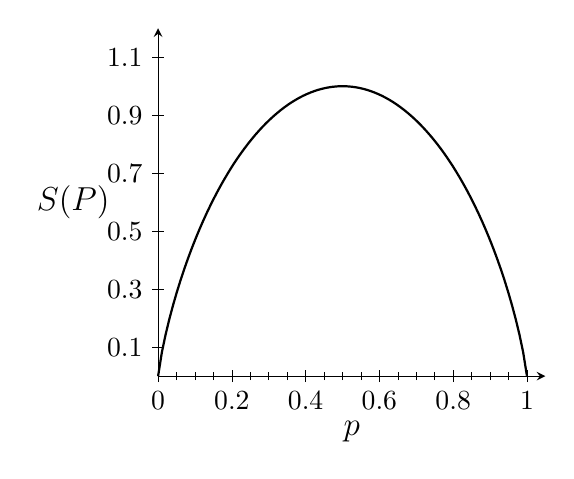
\begin{tikzpicture}
        \begin{axis}[
            width=6.5cm, height=6cm,
            axis lines=left,
            % Rango de los ejes
            xmin=0, xmax=1.05,
            ymin=0, ymax=1.2,
            % Estilo de los ticks (marcas en los ejes)
            xtick={0, 0.2, 0.4, 0.6, 0.8, 1},
            ytick={0.1, 0.3, 0.5, 0.7, 0.9, 1.1},
            minor xtick={0.05,0.1,...,1}, % Ticks pequeños
            tick style={black},
            % Etiquetas de los ejes
            xlabel={$p$},
            ylabel={$S(P)$},
            x label style={at={(axis description cs:0.5,-0.1)},anchor=north, font=\large},
            y label style={at={(axis description cs:-0.1,0.5)},rotate=-90,anchor=east, font=\large},
            % Quitar el marco decorativo
            axis line style={-stealth},
            % Muestreo y dominio
            domain=0:1,
            samples=100,
            clip=false
        ]
            % Curva continua: p log p + (1-p) log(1-p)
            \addplot [thick, black] { - (x * log2(x) + (1 - x) * log2(1 - x)) };
        \end{axis}
        \end{tikzpicture}
        \caption{Entropía de Shannon para v.a. $X\sim Ber(p)$}
        \label{fig:entropia_bernoulli}
    \end{figure}
\end{ejemplo}

\noindent
Ahora vamos a ver como maximizar la entropía de Shannon bajo ciertas restricciones, usando el \textit{método de los multiplicadores de Lagrange}, pero, ¿por qué se hace esto? Porque el \tbf{Principio de Máxima Entropía} establece que la mejor distribución que podemos elegir es aquella que maximiza la incertidumbre (Entropía de Shannon) lo que es equivalente a encontrar la distribución de probabilidad más "imparcial" o "uniforme" posible, sujeta a lo que ya sabemos (los vínculos o restricciones). Esto es útil en situaciones donde queremos evitar introducir sesgos innecesarios en nuestras inferencias estadísticas. \\

\noindent
Dado por tanto la definición de entropía de Shannon para una v.a. continua, vamos a intentar maximizarla bajo las siguientes restricciones
\begin{itemize}
    \item Para obtener una función de densidad de probabilidad válida, la integral de la función de densidad debe ser igual a 1, es decir,
    \begin{equation*}
        \int p(x) dx = 1
    \end{equation*}
\end{itemize}
a estas restricciones podemos añadir otras adicionales, que se conozcan del problema en cuestión, como por ejemplo
\begin{itemize}
    \item La media de la distribución es igual a un valor conocido $\mu$, es decir,
    \begin{equation*}
        \int x p(x) dx = \mu
    \end{equation*}
    \item La varianza de la distribución es igual a un valor conocido $\sigma^2$, es decir,
    \begin{equation*}
        \int (x - \mu)^2 p(x) dx = \sigma^2
    \end{equation*}
\end{itemize}
pero para el desarrollo que haremos a continuación, solo usaremos la primera restricción, que es la que conocemos en general siempre, y desarrollaremos lo que se llama \tbf{Optimización con restricciones} (extremizzazione vincolata) usando el \underline{método de los multiplicadores de Lagrange}. Veámoslo

\begin{equation*}
    \widehat{S}_{\lambda}(P) = S+\lambda\left( \int p(x) dx -1 \right)= -k \int p(x) \log p(x) dx + \lambda \left( \int p(x) dx -1 \right)
\end{equation*}
COPIAR DESARROLLO Y EXPLICACIÓN. \\
% //TODO: copiar desarrollo y explicación Jesus

\noindent
Finalmente, el resultado de este desarrollo es que la distribución que maximiza la entropía de Shannon bajo la restricción de que la integral de la función de densidad es igual a 1, es la distribución uniforme en el intervalo considerado. Esto tiene sentido intuitivamente, ya que la distribución uniforme es la que tiene la mayor incertidumbre posible dentro de un intervalo dado, ya que todos los resultados son igualmente probables. \\
\noindent
Tenemos por tanto que para un problema con soporte en el intervalo $[a,b]$ sin conocer nada más, la distribución que maximiza la entropía de Shannon es
\begin{equation*}
    p(x) = \dfrac{1}{b-a} \quad x \in [a,b]
\end{equation*}
es decir, la distribución uniforme en $[a,b]$, $X\sim \cc{U}(a,b)$. \\ \\
\noindent
Ahora vamos a ver otro ejemplo, en este caso añadiendo las restricciones de media y varianza conocidas, y obtener por tanto la distribución que maximiza la entropía de Shannon bajo estas restricciones. \\ \\

\noindent
COPIAR DESARROLLO Y EXPLICACIÓN. \\
% //TODO: copiar desarrollo y explicación Jesus

\noindent
Finalmente, el resultado de este desarrollo es que la distribución que maximiza la entropía de Shannon bajo las restricciones de media y varianza conocidas, es la distribución normal con dicha media y varianza. Esto tiene sentido intuitivamente, ya que la distribución normal es la que tiene la mayor incertidumbre posible dado un valor fijo de media y varianza. \\
\noindent
Tenemos por tanto que para un problema con media $\mu$ y varianza $\sigma^2$ conocidas, la distribución que maximiza la entropía de Shannon es
\begin{equation*}
    p(x) = \dfrac{1}{\sqrt{2\pi \sigma^2}} \exp\left( -\dfrac{(x-\mu)^2}{2\sigma^2} \right) \quad x \in \mathbb{R}
\end{equation*}
es decir, la distribución normal, $X\sim \cc{N}(\mu,\sigma^2)$. \\

\begin{definicion}[Cross entropy]
    Dadas dos distribuciones de probabilidad $p$ y $q$ sobre el mismo espacio de eventos, la \tbf{entropía cruzada} entre las dos distribuciones calcula el error que cometo al usar la distribución $p$ para aproximar la distribución real $q$. Se define como
    \begin{equation*}
        H(q, p) = - \sum\limits_{i} q(x_i) \log p(x_i)
    \end{equation*}
    en el caso discreto, y como
    \begin{equation*}
        H(q, p) = - \int_{X} q(x) \log p(x) dx
    \end{equation*}
    en el caso continuo.
\end{definicion}
\noindent
En nuestro caso concreto, cuando trabajamos con un problema de datos supervisados, es decir, $D=\{(x_i,y_i)\}_{i=1}^{n}$, y tenemos una distribución de probabilidad $P$ con la que queremos aproximar la distribución real de los datos $Q$, usando la función de log-verosimilitud tenemos que 

% //TODO: copiar y explicar mejor el porque de esto (apuntes Jesus e Ilaria)
\begin{align*}
    \ell(\theta; D) &= \dfrac{1}{n} \sum_{i} \log P_{\theta}(y_i \mid x_i) \approx_{n\to \infty} \int q(x,y) \log P_{\theta}(y \mid x) dx dy = \\
    &= \int q(x) \left( \underbrace{\int q(y\mid x) \log P_{\theta}(y \mid x) dy}_{CE[Q,P]} \right) dx \Longrightarrow \ell(\theta; D) \approx - \int q(x) CE[Q,P] dx
\end{align*}
donde hemos usado que los datos $(x_i,y_i)$ son i.i.d. según la distribución real $Q$, y por tanto, $q(x,y) = q(x) q(y\mid x)$. Tenemos entonces que maximizar la función de log-verosimilitud es equivalente a minimizar la entropía cruzada entre la distribución real $Q$ y la distribución del modelo $P_{\theta}$. \\


\section{Distribución Gaussiana multivariante}
\begin{definicion}[Difeomorfismo]
    Sea $X\subseteq R^n$ un abierto. Una función $g: X \to Y \subseteq R^n$ es un \tbf{difeomorfismo} si es biyectiva, diferenciable y su inversa $g^{-1}: Y \to X$ también es diferenciable.
\end{definicion}

\begin{prop}[Transformazioni di densità]
    Sea $X\subseteq R^n$ un abierto y $P$ una distribución de probabilidad en $(X, \cc{B}_X)$ con función de densidad $p(x)$. Sea $g: X \to Y \subseteq R^n$ un difeomorfismo de clase $C^1$, entonces la distribución de probabilidad $P \circ g^{-1}$ en $Y$ tiene función de densidad
    \begin{equation*}
        q(y) = p(g^{-1}(y)) \left| \det J_{g^{-1}}(y) \right| \quad \forall y \in Y
    \end{equation*}
    donde $J_{g^{-1}}(y)$ es la matriz jacobiana de la función $g^{-1}$ evaluada en $y$.
    \begin{proof}
        % //TODO: copiar y entender demostración Jesus, Cristian y Ilaria
    \end{proof}
\end{prop}

\begin{teo}[Vettore di gaussiane standard]
    Sean $X_1, X_2, \ldots, X_n$ v.a.s independientes e idénticamente distribuidas según una distribución normal estándar, $X_i \sim \cc{N}(0,1)$. Dado $B\in \R^{n\times n}$ una matriz invertible y $m\in \R^n$ un vector, entonces la v.a. $Y=BX + m$ tiene función de densidad
    \begin{equation*}
        p_Y(y) = \dfrac{1}{(2\pi)^{n/2} \sqrt{|\det(C)|}} \exp\left( -\dfrac{1}{2} (x - m)^T C^{-1} (x - m) \right)
    \end{equation*}
    donde $C:=B B^T$ y $X=(X_1, X_2, \ldots, X_n)^T$.
    \begin{proof}
        % //TODO: copiar y entender demostración Jesus, Cristian y Ilaria
    \end{proof}
\end{teo}

\begin{observacion}
    En el teorema anterior, la matriz $C$ es simétrica y definida positiva.
\end{observacion}

\begin{definicion}[Matriz definida positiva]
    Una matriz simétrica $C \in \R^{n\times n}$ se dice \tbf{definida positiva} si $\forall v\in \R^n, v\neq 0$ se cumple que
    \begin{equation*}
        v^T C v > 0
    \end{equation*}
\end{definicion}

\begin{prop}[Caracterización de matrices definidas positivas]
    Una matriz es definida positiva si y solo si todos sus autovalores son estrictamente positivos ($\lambda_i > 0$ para todo $i$)
\end{prop}

\begin{definicion}[Gaussiana multivariata]
    Dada una v.a. $Y=(Y_1, Y_2, \ldots, Y_n)^T$ se dice \tbf{variable aleatoria gaussiana multivariante} si $\exists m\in \R^n, \exists C\in \R^{n\times n}$ simétrica y definida positiva tal que distribución de $Y$ tiene función de densidad 
    \begin{align*}
        p_Y(y) = \dfrac{1}{(2\pi)^{n/2} \sqrt{|\det(C)|}} \exp\left( -\dfrac{1}{2} (x - m)^T C^{-1} (x - m) \right)
    \end{align*}
    y se escribe $Y \sim \cc{N}(m, C)$.
\end{definicion}

\begin{observacion}
    Si $Y\sim \cc{N}_n(m,C)$, entonces 
    \begin{equation*}
        \E[Y_i]=m \quad \text{y} \quad Cov(Y_i,Y_j)=C_{ij} \quad  i,j=1,2,\ldots,n
    \end{equation*}
\end{observacion}

\begin{prop}
    Sea $Y\sim \cc{N}_n(m,C)$ una v.a. gaussiana multivariante con $C$ matriz simétrica y definida positiva, entonces $\exists X\sim \cc{N}_n(0,I_n)$ tal que 
    \begin{equation*}
        Y = B X + m
    \end{equation*}
    donde $C=BB^T$, es decir, $B=\sqrt{C}$.
\end{prop}

\section{Distribuciones relacionadas con la normal}

\subsubsection{Distribución Gamma}
\noindent
Previamente al estudio de la distribución Gamma, vamos a estudiar la función Gamma, que es la función que da nombre a la distribución.
Esta es:
\Func{\Gamma}{\bb{R}^+}{\bb{R}^+}{x}{\displaystyle \int_{0}^{\infty} t^{x-1}e^{-t}~dt}


Algunas propiedades son:
\begin{enumerate}
    \item $\Gamma(1) = 1$. \label{prop:gamma1}
    \item $\Gamma(x+1) = x\Gamma(x),\qquad \forall x\in \bb{R}^+$. \label{prop:gamma2}
    \item $\Gamma(n) = (n-1)!,\qquad \forall n\in \bb{N}$. \label{prop:gamma3}
\end{enumerate}

\begin{definicion}
    Dada $X$ una variable aleatoria y $\alpha,r>0$, se dice que $X$ sigue una \tbf{distribución gamma} con parámetros $\alpha$ y $r$ si $\Gamma_{\alpha,r}$ es una medidad de probabilidad en $(\R^+, \cc{B}(\R^+))$ con función de densidad
    \begin{equation*}
        p_{\alpha,r}(x) = \dfrac{\alpha^r}{\Gamma(r)} x^{r - 1} e^{-\alpha x} \quad x> 0
    \end{equation*}
    donde $\Gamma(r) = \int_0^{\infty} t^{r - 1} e^{-t} dt$ es la función gamma, y se denota como $X \sim \Gamma(\alpha,r)$.
\end{definicion}

\subsubsection{Distribución $\chi^2$}

\begin{definicion}
    Dada $X$ una variable aleatoria, se dice que $X$ sigue una \tbf{distribución chi-cuadrado} si $X$ tiene distribución gamma con parámetros $\alpha = 1/2$ y $r = 1/2$, es decir, \mbox{$\chi^2 = \Gamma_{\dfrac{1}{2}, \dfrac{1}{2}}$}. La función de densidad es
    \begin{equation*}
        p_{1/2,1/2}(x) = \dfrac{1}{\sqrt{2}\Gamma(1/2)} x^{-1/2} e^{-x/2} \quad x> 0
    \end{equation*}
    y se denota como $X \sim \chi^2$.
\end{definicion}

\begin{definicion}
    Dada $X$ una variable aleatoria, se dice que $X$ sigue una \tbf{distribución chi-cuadrado con $n$ grados de libertad} si $X$ tiene distribución gamma con parámetros $\alpha = 1/2$ y $r = n/2$, es decir, $\chi^2_n = \Gamma_{1/2, n/2}$. La función de densidad es
    \begin{equation*}
        p_{1/2,n/2}(x) = \dfrac{1}{2^{n/2}\Gamma(n/2)} x^{(n/2) - 1} e^{-x/2} \quad x> 0
    \end{equation*}
    y se denota como $X \sim \chi^2_n$.
\end{definicion}

\begin{prop}
    Sea $X \sim \cc{N}(0,1)$ una variable aleatoria con distribución normal estándar, entonces la variable aleatoria $Y = X^2$ sigue una distribución chi-cuadrado, es decir, $Y \sim \chi^2$.
    \begin{proof}
        % //TODO: copiar y entender demostración Jesus, Cristian y Ilaria
    \end{proof}
\end{prop}

\begin{teo}
    Sean $X_1, X_2, \ldots, X_n$ v.a.s independientes e idénticamente distribuidas según una distribución normal estándar, $X_i \sim \cc{N}(0,1)$. Entonces la variable aleatoria 
    \begin{equation*}
        \sum\limits_{i=1}^{n} X_i^2 \sim \Gamma\left( \dfrac{1}{2}, \dfrac{n}{2} \right)=\chi_n^2
    \end{equation*}
    \begin{proof}
        % //TODO: copiar demostración Jesus, Cristian y Ilaria
    \end{proof}
\end{teo}

\subsubsection{Distribución Beta}

\begin{definicion}[Función Beta]
    La \tbf{función Beta de Euler} es una función definida como:
    \Func{\beta}{\bb{R}^+ \times \bb{R}^+}{\bb{R}^+}{(p,q)}{\displaystyle \int_{0}^{1} t^{p-1}(1-t)^{q-1}~dt}
\end{definicion}

Algunas propiedades son:
\begin{enumerate}
    \item Es simétrica. Es decir, $\forall p,q\in \bb{R}^+$, se cumple que $\beta(p,q) = \beta(q,p)$.
    \item $\beta(p,q) = \dfrac{\Gamma(p)\Gamma(q)}{\Gamma(p+q)}$.  
\end{enumerate}

\begin{definicion}[Distribución Beta]
    Una variable aleatoria continua $X$ sigue una \tbf{distribución Beta} con parámetros $p,q\in \bb{R}^+$ en $]0,1[$, si su función de densidad es:
    \begin{equation*}
        f_X(x) = \dfrac{1}{\beta(p,q)}x^{p-1}(1-x)^{q-1} \quad  x\in [0,1]
    \end{equation*}
    Lo denotaremos como $X\sim \beta(p,q)$.
\end{definicion}

\begin{prop}
    Dados $r,s>0$ y $X\sim \Gamma(\alpha,r)$, $Y\sim \Gamma(\alpha,s)$ dos variables aleatorias independientes, entonces
    \begin{equation*}
        X+Y \sim \Gamma(\alpha, r+s) \quad \text{y} \quad \dfrac{X}{X+Y} \sim \beta(r,s)
    \end{equation*}
    \begin{proof}
        % //TODO: copiar y entender demostración Jesus, Cristian y Ilaria
    \end{proof}
\end{prop}

\subsubsection{Distribución t-Student}
\begin{definicion}
    Una variable aleatoria $X$ sigue una \tbf{distribución t-Student con $n$ grados de libertad} sobre $]0,+\infty[$ si su función de densidad es
    \begin{equation*}
        \tau_n(x) =  \left( 1 + \dfrac{x^2}{n} \right)^{-\dfrac{n+1}{2}} \left(\sqrt{n}B\left(\dfrac{1}{2},\dfrac{n}{2}\right)\right)^{-1} \quad x\in \R^+
    \end{equation*}
    y se denota como $X \sim t_n$.
\end{definicion}

\begin{coro}
    Sean las variables aleatorias $X, Y_1, \ldots, Y_n$ i.i.d. con distribución común $\cc{N}(0,1)$, entonces 
    \begin{equation*}
        Z = \dfrac{X}{\sqrt{\dfrac{1}{n} \sum\limits_{i=1}^{n} Y_i^2}} \sim t_n
    \end{equation*}
    \begin{proof}
        % //TODO: copiar y entender demostración Jesus, Cristian y Ilaria
    \end{proof}
\end{coro}

\begin{teo}
    Sea el modelo estadístico de producto gaussiano n-ario
    \begin{equation*}
        (\R^n , B(\R^n) , N_{m,v}^{\otimes n} ; m \in \R, v>0)
    \end{equation*}
    y sean las v.a.s. $(X_i)_{i=1}^{n}$ como las proyecciones, es decir, son i.i.d. y $X_i\sim \cc{N}(m,v)$. Definimos las siguientes variables aleatorias
    \begin{align*}
        M = \dfrac{1}{n} \sum\limits_{i=1}^{n} X_i \quad , \quad V^* = \dfrac{1}{n} \sum\limits_{i=1}^{n-1} (X_i - M)^2 
    \end{align*}
    las siguientes afirmaciones son ciertas
    \begin{itemize}
        \item $M$ y $V^*$ son independientes.
        \item $M \sim N(m, \dfrac{v}{n})$ y $\dfrac{n-1}{v} V^* \sim \chi^2_{n-1}$.
        \item $\dfrac{\sqrt{n} (M - m)}{\sqrt{V^*}} \sim t_{n-1}$.
    \end{itemize}
\end{teo}

\section{Teorema de estimación de Cramér-Rao-Fisher}

\begin{definicion}[Modello statistico regolare]
    Sea un modelo estadístico $(X, \cc{B}_{X}, P_{\theta}; \theta \in \Theta)$ con función de densidad $p_{\theta}(x)$ y $\Theta\subseteq \R$, se dice que es un \tbf{modelo estadístico regular} si se cumplen las siguientes condiciones:
    \begin{enumerate}[label=(\arabic*)]
        \item $\Theta$ es un abierto en $\R$.
        \item $p_{\theta}(x)$ es estrictamente positiva y continuamente diferenciable respecto a $\theta$. En particular, existe la función llamada \tbf{función de puntuación} (score function)
        \begin{equation*}
            U_{\theta}(x) = \dfrac{d}{d\theta} \log p_{\theta}(x)
        \end{equation*}
        \item $p$ permite intercambiar la diferenciación respecto a $\theta$ y la integración sobre $x$, es decir,
        \begin{equation*}
            \dfrac{d}{d\theta} \int_{X} p_{\theta}(x) dx = \int_{X} \dfrac{d}{d\theta} p_{\theta}(x) dx
        \end{equation*}
        (como siempre para $X$ discreto la integral se sustituye por una suma).
        \item Para cada $\theta \in \Theta$, la varianza $I(\theta) := V_{\theta} \left( U_{\theta} \right)$ existe y no es nula.
    \end{enumerate}
    La función $I:\theta\to I(\theta)$ se llama \tbf{información de Fisher}.
\end{definicion}

\begin{prop}
    Sea un modelo estadístico regular $(X, \cc{F}, P_{\theta}; \theta \in \Theta)$, entonces se cumple que
    \begin{equation*}
        \E_{\theta} \left[ U_{\theta} \right] = 0 \quad \text{y} \quad I(\theta) = -\E_{\theta} \left[ \dfrac{d}{d\theta} U_{\theta} \right]= -\E_{\theta}\left[\dfrac{d^2}{d\theta^2}\log p_{\theta}\right]
    \end{equation*}
    \begin{proof}
        Primero vamos a demostrar que $\E_{\theta} \left[ U_{\theta} \right] = 0$. Por definición de esperanza tenemos que
        \begin{align*}
            \E_{\theta} \left[ U_{\theta} \right] &= \E\left[\dfrac{d}{d\theta} \log p_{\theta}(X)\right] = \int_{X} \dfrac{d}{d\theta} \log p_{\theta}(x) p_{\theta}(x) dx= \int_{X} \dfrac{p'_\theta(x)}{p_{\theta}(x)}p_{\theta}(x) dx = \\
            &= \int_{X} p'_{\theta}(x) dx \overset{(*)}{=} \dfrac{d}{d\theta} \int_{X} p_{\theta}(x) dx = \dfrac{d}{d\theta} 1 = 0
        \end{align*}
        donde en $(*)$ hemos usado la propiedad (3) de modelo estadístico regular y en la última igualdad hemos usado que la integral de una función de densidad es 1. \\
        Veámos ahora la segunda igualdad
        \begin{align*}
            0&=\dfrac{d}{d\theta}\int_{X}p_{\theta}(x) \dfrac{d}{d\theta} \log p_{\theta}(x)  dx \overset{(3)}{=} \int_{X} \dfrac{d}{d\theta} \left( p_{\theta}(x) \dfrac{d}{d\theta} \log p_{\theta}(x) \right) dx =  \\
            &\overset{(*)}{=}\int_{X}  \dfrac{d}{d\theta} p_{\theta}(x) \dfrac{d}{d\theta} \log p_{\theta}(x)dx + \int_{X}p_{\theta}(x) \dfrac{d^2}{d\theta^2} \log p_{\theta}(x) dx = \\
            &= \underbrace{\int_{X}  U_{\theta}(x)p_{\theta}(x)U_{\theta}(x) dx}_{I(\theta)} + \int_{X}p_{\theta}(x) \dfrac{d^2}{d\theta^2} \log p_{\theta}(x) dx=0 \Longrightarrow \\
            & \overset{(**)}{\Longrightarrow} I(\theta)= -\E_{\theta}\left[\dfrac{d^2}{d\theta^2}\log p_{\theta}\right]=-\E_{\theta} \left[ \dfrac{d}{d\theta} U_{\theta} \right]
        \end{align*}
        donde en $(*)$ hemos usado la regla del producto para derivadas y en $(**)$ hemos usado que por el resultado anterior ahora sabemos que $I(\theta)=\E[U_{\theta}^2]$.
    \end{proof}
\end{prop}

\begin{prop}[Aditividad de la información de Fisher]
    Sea un modelo estadístico regular $(X, \cc{B}_{X}, P_{\theta}; \theta \in \Theta)$ con información de Fisher $I(\theta)$. Entonces el modelo estadístico de producto n-ario
    \begin{equation*}
        (X^n, \cc{F}^{\otimes n}, P_{\theta}^{\otimes n}; \theta \in \Theta)
    \end{equation*}
    es un modelo estadístico regular con información de Fisher
    \begin{equation*}
        I_n(\theta) = n I(\theta)
    \end{equation*}
    donde además la función de puntuación del modelo estadístico de producto n-ario es
    \begin{equation*}
        U_{\theta}^{(n)}(x_1, x_2, \ldots, x_n) = \sum\limits_{i=1}^{n} U_{\theta}(x_i)
    \end{equation*}
\end{prop}

\begin{ejemplo}
    \begin{enumerate}
        \item Sea $X\sim \cc{N}(\mu, \sigma^2)$ una variable aleatoria, donde conocemos $\sigma^2$ y queremos estimar $\mu$, es decir, tenemos el modelo estadístico
        \begin{equation*}
            (\R, B(\R), N_{\mu,\sigma^2}; \mu \in \R)
        \end{equation*}
        El modelo estadístico es regular, y para poder obtener la información de Fisher tenemos que calcular la función de puntuación
        \begin{align*}
            p_{\mu}(x)=\dfrac{1}{\sqrt{2\pi \sigma^2}} \exp\left( -\dfrac{(x-\mu)^2}{2\sigma^2} \right) \quad &\Longrightarrow \quad \log p_{\mu}(x) = -\dfrac{1}{2} \log(2\pi \sigma^2) - \dfrac{(x-\mu)^2}{2\sigma^2}  \Longrightarrow\\
            & \Longrightarrow U_{\mu}(x) = \dfrac{d}{d\mu} \log p_{\mu}(x) = \dfrac{x-\mu}{\sigma^2}
        \end{align*}
        Calculada la función de puntuación, obtengamos la información de Fisher
        \begin{equation*}
            I(\mu)= \E[U_{\mu}^2]=\E\left[\dfrac{(X-\mu)^2}{\sigma^4}\right]=\dfrac{1}{\sigma^4}\E[(X-\mu)^2]=\dfrac{\sigma^2}{\sigma^4}=\dfrac{1}{\sigma^2} 
        \end{equation*}
        Para el caso del modelo estadístico de producto n-ario, tenemos que la información de Fisher es
        \begin{equation*}
            I_n(\mu) = n I(\mu) = \dfrac{n}{\sigma^2}= \dfrac{1}{\sigma^2/n}= \dfrac{1}{Var(\bar{X})}=\dfrac{1}{\sigma_{\bar{X}}^2}
        \end{equation*}
        \item Sea $X\sim Ber(p)$ una variable aleatoria, donde queremos estimar $p$, es decir, tenemos el modelo estadístico
        \begin{equation*}
            (\{0,1\}, \cc{P}(\{0,1\}), Ber(p); p \in (0,1))
        \end{equation*}
        El modelo estadístico es regular, y sabemos que $P(X=1)=p$ y $P(X=0)=1-p$. Por tanto, para poder obtener la información de Fisher tenemos que calcular la función de puntuación 
        \begin{align*}
            &U_p(X=1)=\dfrac{d}{dp} \log P(X=1)=\dfrac{d}{dp} \log p = \dfrac{1}{p} \\
            &U_p(X=0)=\dfrac{d}{dp} \log P(X=0)=\dfrac{d}{dp} \log(1-p) = -\dfrac{1}{1-p}
        \end{align*}
        entonces la información de Fisher es
        \begin{align*}
            I(p) &= \E[U_p^2] = P(X=1) U_p(X=1)^2 + P(X=0) U_p(X=0)^2 = p \left( \dfrac{1}{p} \right)^2 + (1-p) \left( -\dfrac{1}{1-p} \right)^2 = \\
            &= \dfrac{1}{p} + \dfrac{1}{1-p} = \dfrac{1}{p(1-p)}
        \end{align*}
        donde como al tratarse de una variable aleatoria discreta, la esperanza se calcula como suma ponderada de las probabilidades. \\
        Si ahora calculamos la entropía de Shannon para esta distribución, tenemos que
        \begin{equation*}
            S(P) = - \sum\limits_{x\in \{0,1\}} P(X=x) \log P(X=x) = -p \log p - (1-p) \log(1-p) 
        \end{equation*}
        podemos observar que la información de Fisher y la entropía de Shannon están relacionadas, ya que se comportan de forma contraria, como bien podemos ver en la Figura \ref{fig:entropia_fisher_bernoulli}. \\
        \noindent
        En este sentido, son inversas en su significado, ya que una mayor entropía implica una mayor incertidumbre en la distribución, lo que a su vez implica una menor información disponible para estimar el parámetro $p$.
        \begin{figure}[H]
            \centering
            \begin{tikzpicture}
            \begin{axis}[
                width=12cm, height=7cm,
                axis lines=left,
                xmin=0, xmax=1,
                % 1. RESTRICCIÓN DE CÁLCULO: Evita que PGF calculé valores astronómicos
                restrict y to domain=0:50, 
                % 2. LÍMITE VISUAL:
                ymin=0, ymax=6, 
                xtick={0, 0.2, 0.4, 0.6, 0.8, 1},
                xlabel={$p$},
                ylabel={Valor},
                axis line style={-stealth},
                % 3. DOMINIO SEGURO: No empezamos en 0 ni acabamos en 1
                domain=0.01:0.99, 
                samples=200,
                legend style={at={(0.5,-0.2)}, anchor=north, legend columns=-1},
                clip=true % Corta lo que se salga del área de dibujo
            ]
                % Entropía (siempre entre 0 y 1, no da problemas)
                \addplot [thick, black] {-(x*ln(x)/ln(2) + (1-x)*ln(1-x)/ln(2))};
                \addlegendentry{Entropía}
        
                % Información de Fisher (la que causa el error)
                \addplot [thick, red, dashed] {1/(x*(1-x))};
                \addlegendentry{Inf. Fisher}
                
            \end{axis}
            \end{tikzpicture}
            \caption{Entropía e Información de Fisher ($X\sim Ber(p)$).}
            \label{fig:entropia_fisher_bernoulli}
        \end{figure}
        \item Sea $X\sim P(\lambda)$ una variable aleatoria, donde queremos estimar $\lambda$, es decir, tenemos el modelo estadístico \\
        \noindent
        NO ESTA TERMINADO.
        % //TODO: copiar de Jesus y Cristian
    \end{enumerate}
\end{ejemplo}

\begin{teo}[Teorema Fisher/Cramer/Rao]
    Sea un modelo estadístico regular \mbox{$(X, \cc{B}_{X}, P_{\theta}; \theta \in \Theta)$} y sea $T_{\tau}$ un estimador insesgado de una característica $\tau: \Theta \to \R$, es decir, $\E_{\theta}[T(X)] = \tau(\theta)$ para todo $\theta \in \Theta$. Entonces se tiene 
    \begin{enumerate}[label=\arabic*)]
        \item Se cumple el \tbf{límite de Cramer-Rao}
        \begin{equation*}
            Var(T_{\tau}) \geq \dfrac{(\tau'(\theta))^2}{I(\theta)} \quad \forall \theta \in \Theta
        \end{equation*}
        En particular, si $\tau(\theta) = \theta$, entonces
        \begin{equation*}
            Var(T_{\tau}) \geq \dfrac{1}{I(\theta)} \quad \forall \theta \in \Theta
        \end{equation*}
        \item Si $Var(T_{\tau}) = \dfrac{(\tau'(\theta))^2}{I(\theta)}$ para todo $\theta \in \Theta$, entonces 
        \begin{equation*}
            T_{\tau}(x) - \tau(\theta) = \dfrac{\tau'(\theta)}{I(\theta)} U_{\theta}(x)
        \end{equation*}
        que equivale a 
        \begin{equation*}
            p_{\theta}(x) = h(x) \exp\left( a(\theta) T_{\tau}(x) - b(\theta) \right)
        \end{equation*}
        que se llama \tbf{familia exponencial respecto al estimador $T_{\tau}$}, donde tenemos
        \begin{align*}
            &a(\theta) = \int \dfrac{I(\theta)}{I'(\theta)} d\theta \\
            &b(\theta) = \log \int_{X} h(x) \exp\left( a(\theta) T_{\tau}(x) \right) dx \\
            &h(x) \text{ función medible oportuna}
        \end{align*}
    \end{enumerate}
    \begin{proof}
        % //TODO: copiar y entender demostración Jesus y Cristian
    \end{proof}
\end{teo}

\noindent
Dado este teorema, tenemos que si podemos representar la función de densidad del modelo estadístico en la forma de familia exponencial respecto al estimador $T_{\tau}$, entonces el estimador es eficiente, es decir, alcanza el límite de Cramer-Rao, y tenemos por tanto (identificando $a,b,h$) lo siguiente
\begin{align*}
    &\tau(\theta)=\dfrac{b'(\theta)}{a'(\theta)}=\E[T_{\tau}] \\
    &I(\theta)=a'(\theta)\tau'(\theta) \\
    &Var(T_{\tau})=\dfrac{(\tau'(\theta))^2}{I(\theta)}
\end{align*}
y en general para $n$ extracciones distintas tenemos
\begin{equation*}
    p_{\theta}^n(x)=(\prod_{i=1}^n h(x_i))\exp\left(a(\theta)\sum_{i=1}^n T_{\tau}(x_i)-b(\theta)\right)
\end{equation*}

\section{Inferenza Bayesiana}
\noindent
Antes de introducir el ejemplo que dará sentido a las siguientes definiciones, recordemos el teorema de Bayes en su forma más simple, es decir, el caso discreto. 

\begin{teo}[Regla de Bayes]
    Sea $(\Omega, \mathcal{A}, P)$ un espacio de probabilidad y sea $\{A_n\}_{n \in \N} \subset \mathcal{A}$ una partición de $\Omega$ con $P(A_n)>0~~\forall n \in \N$. Entonces, $\forall B \in \mathcal{A}$:
    $$P(A_j \mid B) = \dfrac{P(B \mid A_j)P(A_j)}{\sum\limits_{i=1}^\infty P(B \mid A_i)P(A_i)}\qquad j \in \N$$
  \end{teo}

\begin{ejemplo}[Seguro de coche]
    Un cliente se acerca a una compañía de seguros para obtener una cita para su nuevo seguro de coche. Tiene un estilo de conducción particular que provoca, con probabilidad $\theta$ $\in [0,1]$, al menos un reclamo por año. Obviamente, el agente de seguros no conoce $\theta$, pero tiene estadísticas sobre las frecuencias de reclamaciones para la población total. Estos le proporcionan una evaluación de riesgo a priori, es decir, una medida de probabilidad $\pi_0$ en $\Theta = [0,1]$, llamada medida de probabilidad a priori. Supongamos por simplicidad que $\pi$ es 'suave', en el sentido de que tiene una densidad de Lebesgue $\alpha$, lo que significa que 
    \begin{equation*}
        \pi_0(\theta)=1 \quad \forall \theta \in [0,1]
    \end{equation*}
    es decir, todas las frecuencias de reclamaciones son igualmente probables a priori. Podemos ver una representación de la función de densidad a priori en la Figura \ref{fig:densidad_apriori_seguro}. \\
    \noindent
    Ahora, el agente de seguros presume (subjetivamente) que la probabilidad de que el cliente tenga $k$ años de reclamaciones en $n$ años está dada por
    \begin{equation*}
        P_n(X=k)=\int_{0}^{1} \pi_0(\theta) B_{n,\theta}(\{k\}) d\theta
    \end{equation*}
    donde $B_{n,\theta}(\{k\})=\binom{n}{k} \theta^k (1-\theta)^{n-k}$ es la función de probabilidad de una distribución binomial con parámetros $n$ y $\theta$. Desarrollemos
    \begin{align*}
        P_n(X=k) &= \int_{0}^{1} \binom{n}{k} \theta^k (1-\theta)^{n-k} d\theta = \binom{n}{k} \int_{0}^{1} \theta^k (1-\theta)^{n-k} d\theta = \\
        &= \binom{n}{k} \beta(k+1, n-k+1) = \binom{n}{k} \dfrac{\Gamma(k+1)\Gamma(n-k+1)}{\Gamma(n+2)} = \\
        &= \dfrac{n!}{k!(n-k)!} \dfrac{k!(n-k)!}{(n+1)!} = \dfrac{1}{n+1}
    \end{align*}
    lo que tiene total sentido, pues el agente de seguros no tiene información sobre el cliente, por lo que todas las frecuencias de reclamaciones son igualmente probables, de modo que sabiendo que $k$ puede tomar valores entre $0$ y $n$, la probabilidad de cada uno es $\frac{1}{n+1}$. Podemos ver una representación gráfica de esta distribución en la Figura \ref{fig:distribucion_reclamaciones_seguro}. \\
    Ahora pasados estos $n$ años, el agente de seguros observa que el cliente ha hecho $x\in\{0,\ldots,n\}$ reclamaciones. ¿Cómo debe actualizar su evaluación de riesgo a priori $\pi_0$? Utilizando el teorema de Bayes, la respuesta es la siguiente: la nueva evaluación de riesgo, llamada evaluación de riesgo a posteriori, es la función de densidad $\pi_X$ que reemplaza a $\pi_0$ y está dada por
    \begin{equation*}
        P(\theta\mid X=x, n)=\pi_X(\theta) = \dfrac{\pi_0(\theta) B_{n,\theta}(\{x\})}{\int_0^{1} \pi_0(p) B_{n,p}(\{x\}) dp}= \dfrac{\binom{n}{x} \theta^x (1-\theta)^{n-x}}{P_n(X=x)} = (n+1) \binom{n}{x} \theta^x (1-\theta)^{n-x}
    \end{equation*}
    Es decir, la evaluación de riesgo a posteriori es la distribución condicional de $\theta$ dado el evento 'el cliente ha hecho $x$ reclamaciones en $n$ años'. De este modo la nueva función de probabilidad es la siguiente
    \begin{align*}
        P(X=l)&=\int_{0}^{1} \pi_X(\theta) B_{n,\theta}(\{l\}) d\theta = (n+1) \binom{n}{x} \binom{n}{l} \int_{0}^{1} \theta^{x+l} (1-\theta)^{2n - (x+l)} d\theta = \\
        & = (n+1) \binom{n}{x} \binom{n}{l} \beta(x+l+1, 2n - (x+l) + 1) 
    \end{align*}
    Veamos ahora la esperanza en ambos casos, es decir, usando ambas funciones de densidad $\pi_0$ y $\pi_X$
    \begin{align*}
        \E_{\pi_0}[\theta] &= \int_{0}^{1} \theta \pi_0(\theta) d\theta = \int_{0}^{1} \theta d\theta = \dfrac{1}{2} \\
        \E_{\pi_X}[\theta] &= \int_{0}^{1} \theta \pi_X(\theta) d\theta = (n+1) \binom{n}{k} \int_{0}^{1} \theta^{x+1} (1-\theta)^{n-x} d\theta = \\
        &= (n+1) \binom{n}{k} \beta(x+2, n-x+1) = (n+1) \binom{n}{x} \dfrac{\Gamma(x+2)\Gamma(n-x+1)}{\Gamma(n+3)} = \\
        &= (n+1) \binom{n}{x} \dfrac{(x+1)! (n-x)!}{(n+2)!} = \dfrac{x+1}{n+2}
    \end{align*}
    Dadas estas dos situaciones (conociendo o no el número de reclamaciones hechas por el cliente), podemos observar que la esperanza de la probabilidad de que el cliente haga una reclamación en un año es $\dfrac{1}{2}$ si no conocemos el número de reclamaciones hechas, mientras que si conocemos que ha hecho $x$ reclamaciones en $n$ años, la esperanza se actualiza a $\dfrac{x+1}{n+2}$, que es una media ponderada entre la esperanza a priori y la frecuencia observada $x/n$. Esto tiene sentido, ya que si el cliente ha hecho muchas reclamaciones, la probabilidad de que haga una en el próximo año debería ser mayor que si no hubiera hecho ninguna. Por tanto, la inferencia bayesiana nos permite actualizar nuestras creencias sobre la probabilidad de que un evento ocurra en función de la evidencia observada. \\ \\
    \noindent
    De hecho, si definimos dos estimadores de la siguiente manera 
    \begin{align*}
        T_{\theta}(X) &= \dfrac{X}{n} \quad \text{(estimador no sesgado)} \\
        S_{\theta}(X) &= \dfrac{X+1}{n+2} \quad \text{(estimador sesgado)}
    \end{align*}
    viendo la gráfica del error cuadrático medio de ambos estimadores en la Figura \ref{fig:ecm_estimadores_seguro}, podemos observar que el estimador sesgado $S_{\theta}$ tiene un error cuadrático medio menor que el estimador no sesgado $T_{\theta}$ para ciertos valores de $\theta$. Esto ilustra cómo la incorporación de información a priori puede mejorar la precisión de las estimaciones en ciertos contextos.
\end{ejemplo}

\begin{figure}
    \centering
    \begin{tikzpicture}
    \begin{axis}[
        width=10cm, height=6cm,
        axis lines=left,
        xmin=0, xmax=1.2,
        ymin=0, ymax=1.2,
        xtick={0, 0.2, 0.4, 0.6, 0.8, 1},
        xlabel={$\theta$},
        ylabel={$\pi_0(\theta)$},
        axis line style={-stealth},
        domain=0:1, 
        samples=200,
        legend style={at={(0.5,-0.25)}, anchor=north, legend columns=-1},
        clip=true % Corta lo que se salga del área de dibujo
    ]
        % Densidad a priori
        \addplot [thick, blue] {1};
        \addlegendentry{Densidad a priori}
    \end{axis}
    \end{tikzpicture}
    \caption{Función de densidad a priori $\pi_0(\theta)$ para el seguro de coche.}
    \label{fig:densidad_apriori_seguro}
\end{figure}

\begin{figure}
    \centering
    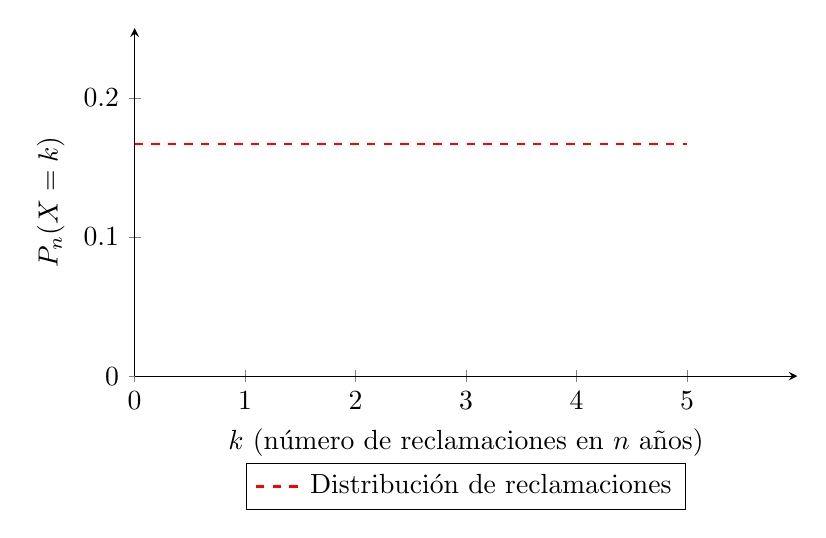
\begin{tikzpicture}
    \begin{axis}[
        width=10cm, height=6cm,
        axis lines=left,
        xmin=0, xmax=6,
        ymin=0, ymax=0.25,
        xtick={0, 1, 2, 3, 4, 5},
        xlabel={$k$ (número de reclamaciones en $n$ años)},
        ylabel={$P_n(X=k)$},
        axis line style={-stealth},
        domain=0:5, 
        samples=200,
        legend style={at={(0.5,-0.25)}, anchor=north, legend columns=-1},
        clip=true % Corta lo que se salga del área de dibujo
    ]
        % Distribución de reclamaciones
        \addplot [thick, red, dashed] {1/6};
        \addlegendentry{Distribución de reclamaciones}
    \end{axis}
    \end{tikzpicture}
    \caption{Distribución de reclamaciones $P_n(X=k)$ para el seguro de coche con $n=5$.}
    \label{fig:distribucion_reclamaciones_seguro}
\end{figure}

\begin{figure}
    \centering
    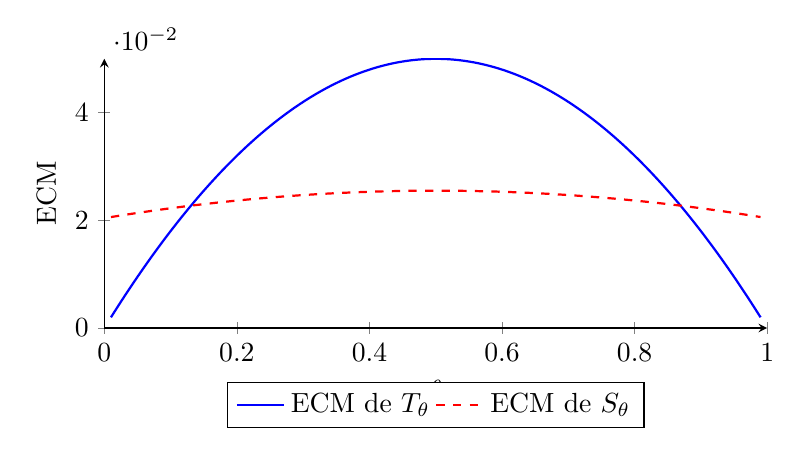
\begin{tikzpicture}
    \begin{axis}[
        width=10cm, height=5cm,
        axis lines=left,
        xmin=0, xmax=1,
        ymin=0, ymax=0.05,
        xtick={0, 0.2, 0.4, 0.6, 0.8, 1},
        xlabel={$\theta$},
        ylabel={ECM},
        axis line style={-stealth},
        domain=0.01:0.99, 
        samples=200,
        legend style={at={(0.5,-0.2)}, anchor=north, legend columns=-1},
        clip=true % Corta lo que se salga del área de dibujo
    ]
        % ECM del estimador no sesgado T0
        \addplot [thick, blue] { (x*(1 - x)) / 5 };
        \addlegendentry{ECM de $T_{\theta}$}
        
        % ECM del estimador sesgado T1
        \addplot [thick, red, dashed] { (( (5*x + 1)/(7) - x )^2 + ( (5*x*(1 - x))/(7^2) )) };
        \addlegendentry{ECM de $S_{\theta}$}
        
    \end{axis}
    \end{tikzpicture}
    \caption{Error cuadrático medio (ECM) de los estimadores $T_0$ y $T_1$ para el seguro de coche con $n=5$.}
    \label{fig:ecm_estimadores_seguro}
\end{figure}

\begin{definicion}[Distribución a priori y a posteriori]
    Sea un modelo estadístico paramétrico estándar \mbox{$(X, \cc{F}, P_{\theta}; \theta \in \Theta)$} con función de probabilidad $p_{\theta}:X\to [0,\infty[$ para cada $\theta\in \Theta$. Entonces, para toda densidad de probabilidad $\pi_0$ en \mbox{$(\Theta, \mathcal{F}')$}, que se llama \tbf{densidad a priori}, y conjunto de datos observados $\{x_1, \ldots, x_n\} \subseteq X$, la \tbf{densidad a posteriori} $\pi_{X}$ está dada por
    \begin{equation*}
        \pi_{X}(\theta) = \dfrac{\pi_0(\theta) \prod\limits_{i=1}^{n} p_{\theta}(x_i)}{\int_{\Theta} \pi_0(p) \prod\limits_{i=1}^{n} p_{p}(x_i) dp}= \dfrac{\pi_0(\theta) L(\theta; D)}{\int_{\Theta} \pi_0(p) L(p; D) dp}= \dfrac{\pi_0(\theta)\exp\left(\dfrac{1}{n} \sum\limits_{i=1}^{n} \log p_{\theta}(x_i)\right)}{\int_{\Theta} \pi_0(p) \exp\left(\dfrac{1}{n} \sum\limits_{i=1}^{n} \log p_{p}(x_i)\right) dp}
    \end{equation*}
\end{definicion}

\begin{observacion}
    Es importante recalcar que $P_{\theta}(X_i)=p_{\theta}(x_i)$ es la función de probabilidad de la variable aleatoria $X_i$ evaluada en el dato observado $x_i$.
\end{observacion}

\begin{definicion}[MSE Bayesiano]
    Sea $(X ; \cc{F} ; P_{\theta}; \theta \in \Theta)$ un modelo estadístico paramétrico estándar con función de verosimilitud $p>0$ que es medible conjuntamente en ambas variables, y sea $\pi$ una distribución a priori en $\Theta$ con densidad $\pi_0$. Además, sea $\tau: X \times \Theta \to \R$ una característica real medible con $E_{\pi_0}(\tau^2) < \infty$. Dado un estimador $T: X \to \R$ de $\tau$ su \tbf{error cuadrático medio (MSE) bayesiano} cuando hay una observación $n=1$ está dado por
    \begin{equation*}
        MSE(T) =\int_{\Theta} \int_{X} (T(x) - \tau(\theta))^2 p_{\theta}(x) dx \pi_0(\theta) d\theta=\dfrac{1}{C} \int_{\Theta} \int_{X} (T(x) - \tau(\theta))^2 \pi_X(\theta) dx d\theta
    \end{equation*}
    Para el caso en el que haya $n>1$ observaciones, el MSE bayesiano se define como
    \begin{align*}
        MSE(T(x_1,\ldots,x_n)) &= \int_{\Theta} \int_{X^n} \prod_{i=1}^n p_{\theta}(x_i)(T(x_1,\ldots,x_n) - \tau(\theta))^2  dx_1 \cdot \ldots\cdot dx_n \pi_0(\theta) d\theta= \\
        &=\dfrac{1}{C}\int_{\Theta} \int_{X^n} (T(D) - \tau(\theta))^2 \pi_D(\theta) dx_1 \cdot \ldots\cdot dx_n  d\theta
    \end{align*}
    donde en ambos casos $C$ es una constante de normalización.
\end{definicion}

\begin{definicion}[Stimatore di Bayes Ottimale]
    En las condiciones anteriores, un estimador $\hat{T}: X \to \R$ se llama \tbf{estimador de Bayes óptimo} (OBE) si minimiza el MSE bayesiano, es decir,
    \begin{equation*}
        \hat{T} = \arg \min_{T} MSE_{\pi_0,p_{\theta}(x)}(T)
    \end{equation*}
    esto equivale a decir que
    \begin{equation*}
        \hat{T}(x) = E_{\pi_X}[\tau(\theta)] = \int_{\Theta} \tau(\theta) \pi_X(\theta) d\theta
    \end{equation*}
    donde $\pi_X$ es la distribución a posteriori dada la muestra observada $X=x$. En muchas ocasiones el estimador de Bayes óptimo se representará como $\theta_{BAYES}$, donde $\theta$ es el parámetro que se está estimando. 
\end{definicion}

\begin{observacion}
    La diferencia clave con el estimador de máxima verosimilitud (MLE) es que el estimador de Bayes óptimo incorpora información a priori sobre el parámetro a través de la distribución a priori $\pi_0$. Esto puede ser especialmente útil cuando se dispone de información previa o cuando los datos son limitados, ya que permite ajustar las estimaciones en función de dicha información adicional, mientras en el caso del estimador MLE solo se basa en los datos observados.
\end{observacion}

\begin{ejemplo}
    % //TODO: copiar y entender Jesus y Cristian
\end{ejemplo}

\begin{definicion}[Función de Dirac]
    La \tbf{función de Dirac} $\delta_a: \R \to \R$ en el punto $a \in \R$ se define como
    \begin{equation*}
        \delta(x-a)=\delta_a(x) = 
        \begin{cases}
            +\infty & x=a \\
            0 & x\neq a
        \end{cases}
    \end{equation*}
    y cumple la propiedad de que
    \begin{equation*}
        \int_{-\infty}^{\infty} f(x) \delta_a(x) dx = f(a)
    \end{equation*}
    para toda función continua $f:\R\to\R$.
\end{definicion}

\begin{prop}
    Una propiedad importante de la función de Dirac es la siguiente:
    $$\delta(g(x)) = \sum_{i} \frac{\delta(x - x_i)}{|g'(x_i)|}$$
    donde los $x_i$ son las raíces de la función $g(x)$.
\end{prop}



% //TODO: copiar y entender resto de información copiad de Jesus y Cristia, es raro porque de sus apuntes de la web no aparece nada